This chapter presents the simulation study results.

\section{SIMULATION STUDY}
\label{cap:simures}

We have seventy-two simulation scenarios where for each one we simulate
300 samples. In total, we fitted 21600 models. The scenarios were
detailed in \autoref{cap:datasets} but let us just recap the parameter
values used.
\begin{description}
 \item[High CIF config.] \(\{\beta_{1} = -2,~\beta_{2} = -1.5,~
                             \gamma_{1} = 1,~\gamma_{2} = 1.5,~
                             w_{1} = 3,~w_{2} = 4\}\);
 \item[Low CIF config.] \(\{\beta_{1} = 3,~\beta_{2} = 2.5,~
                            \gamma_{1} = 2.6,~\gamma_{2} = 4,~
                            w_{1} = 5,~w_{2} = 10\}\).
\end{description}
\begin{minipage}{0.1\textwidth}
 \begin{align*}
  \sigma_{u_{1}}^{2}   &= 1\\
  \sigma_{u_{2}}^{2}   &= 0.7,\\
  \sigma_{\eta_{1}}^{2} &= 0.6\\
  \sigma_{\eta_{2}}^{2} &= 0.9
 \end{align*}
\end{minipage}%
\begin{minipage}{0.9\textwidth}
 \[
  \text{Correlation structure}~=~\begin{blockarray}{ccccc}
                                  u_{1} & u_{2} & \eta_{1} & \eta_{2}\\
                                  \begin{block}{(cccc)c}
                                   1 & 0.1 & -0.5 &  0.3 & u_{1}\\
                                     &   1 &  0.3 & -0.4 & u_{2}\\
                                     &     &    1 &  0.2 & \eta_{1}\\
                                     &     &      &    1 & \eta_{2}\\
                                  \end{block}
                                 \end{blockarray}.
 \]
\end{minipage}

\vspace{0.3cm}
\noindent
The parameter values per se are not important. What is important is keep
in mind

\begin{figure}[H]
 \setlength{\abovecaptionskip}{.0001pt}
 \caption{PARAMETER \(\beta_{1}\) BIAS WITH \(\pm\) 1.96 STANDARD
          DEVIATIONS}
 \vspace{0.2cm}\centering
 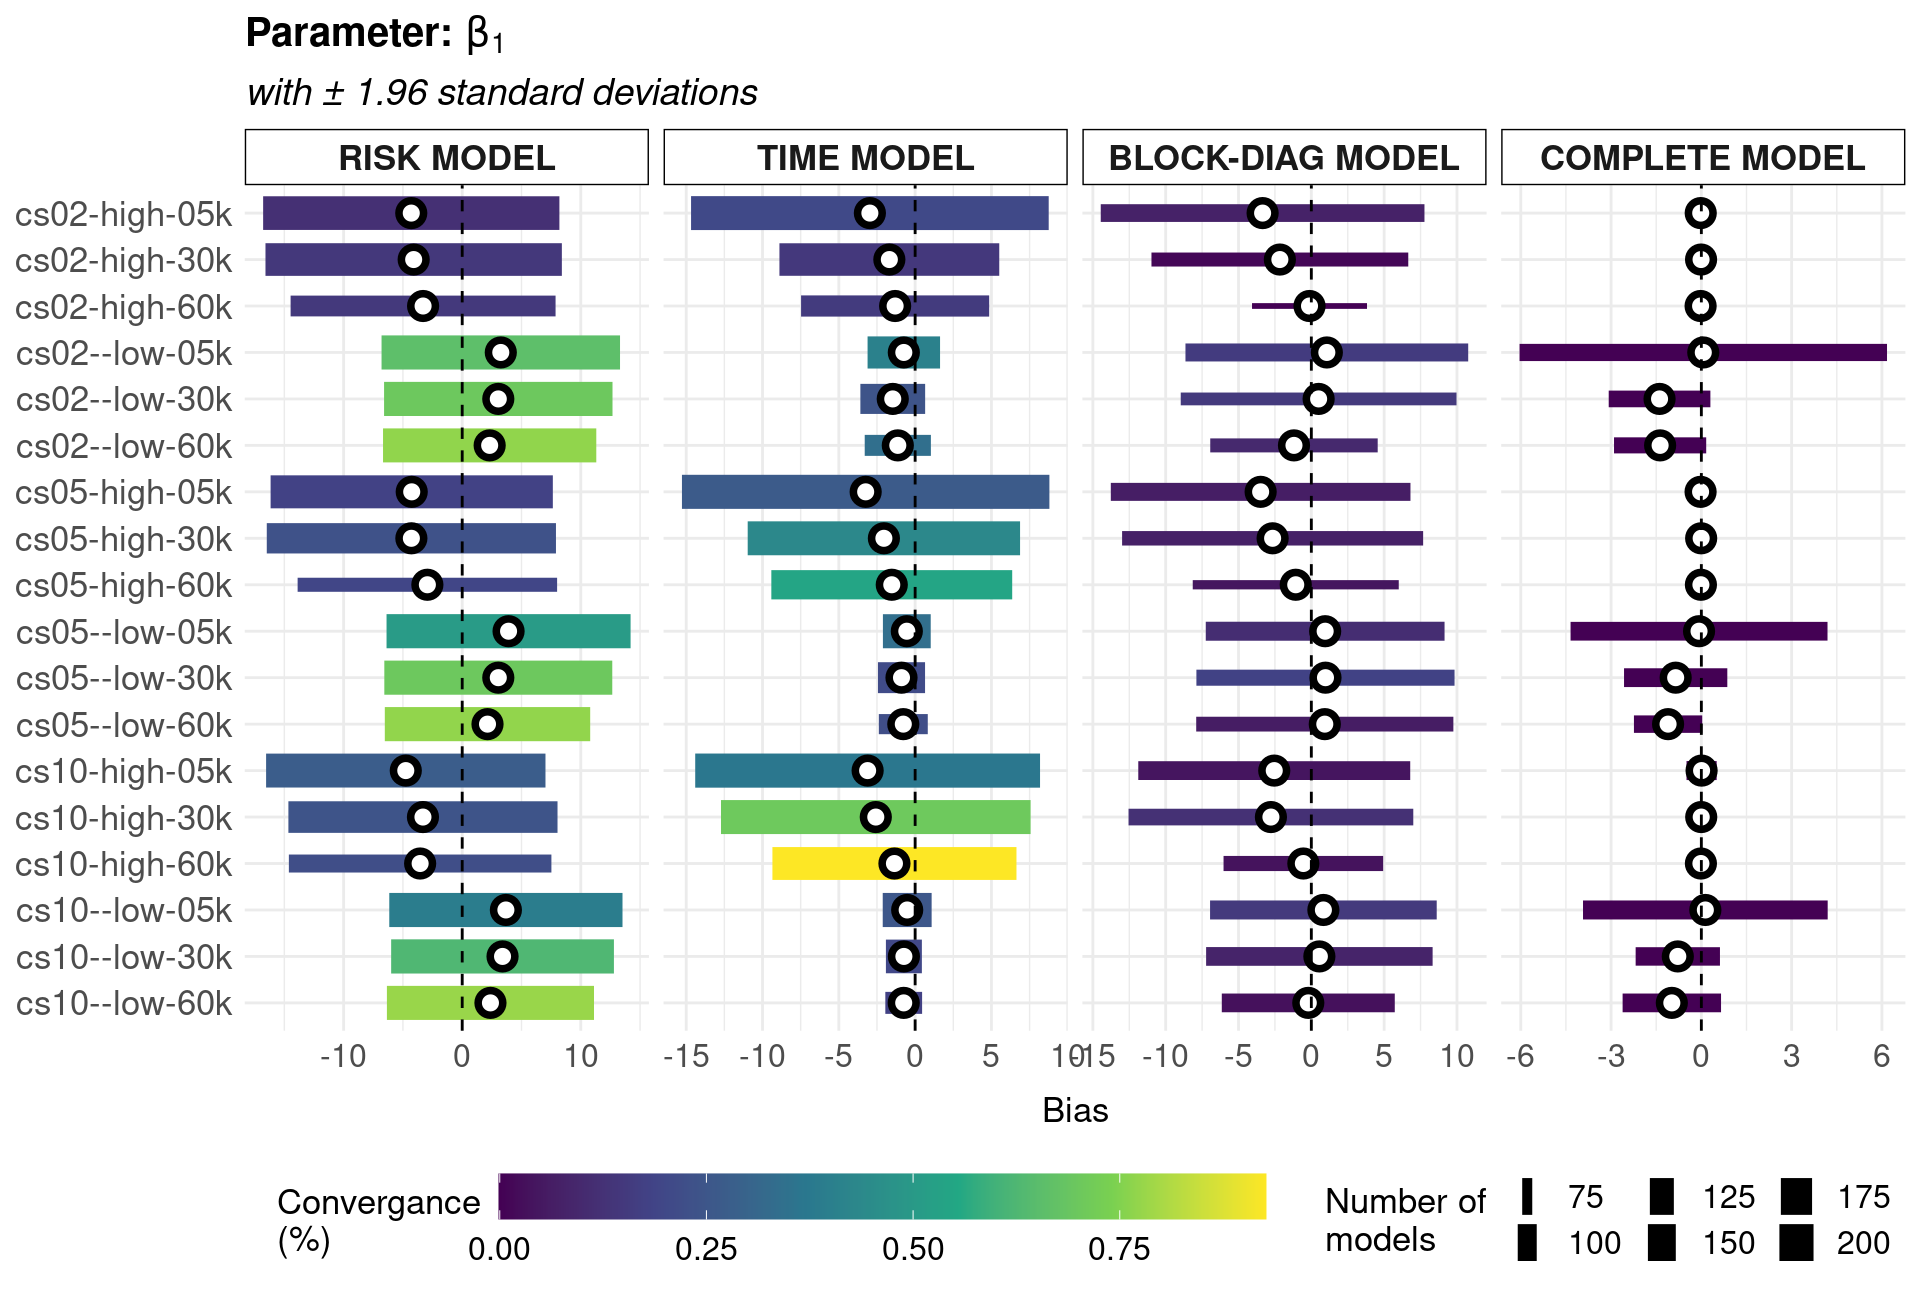
\includegraphics[width=\textwidth]{bias2plotsd-1.png}\\
 \begin{footnotesize}
  SOURCE: The author (2021).
 \end{footnotesize}
 \label{fig:biassdbeta1}
\end{figure}

\begin{figure}[H]
 \setlength{\abovecaptionskip}{.0001pt}
 \caption{PARAMETER \(\beta_{2}\) BIAS WITH \(\pm\) 1.96 STANDARD
         DEVIATIONS}
 \vspace{0.2cm}\centering
 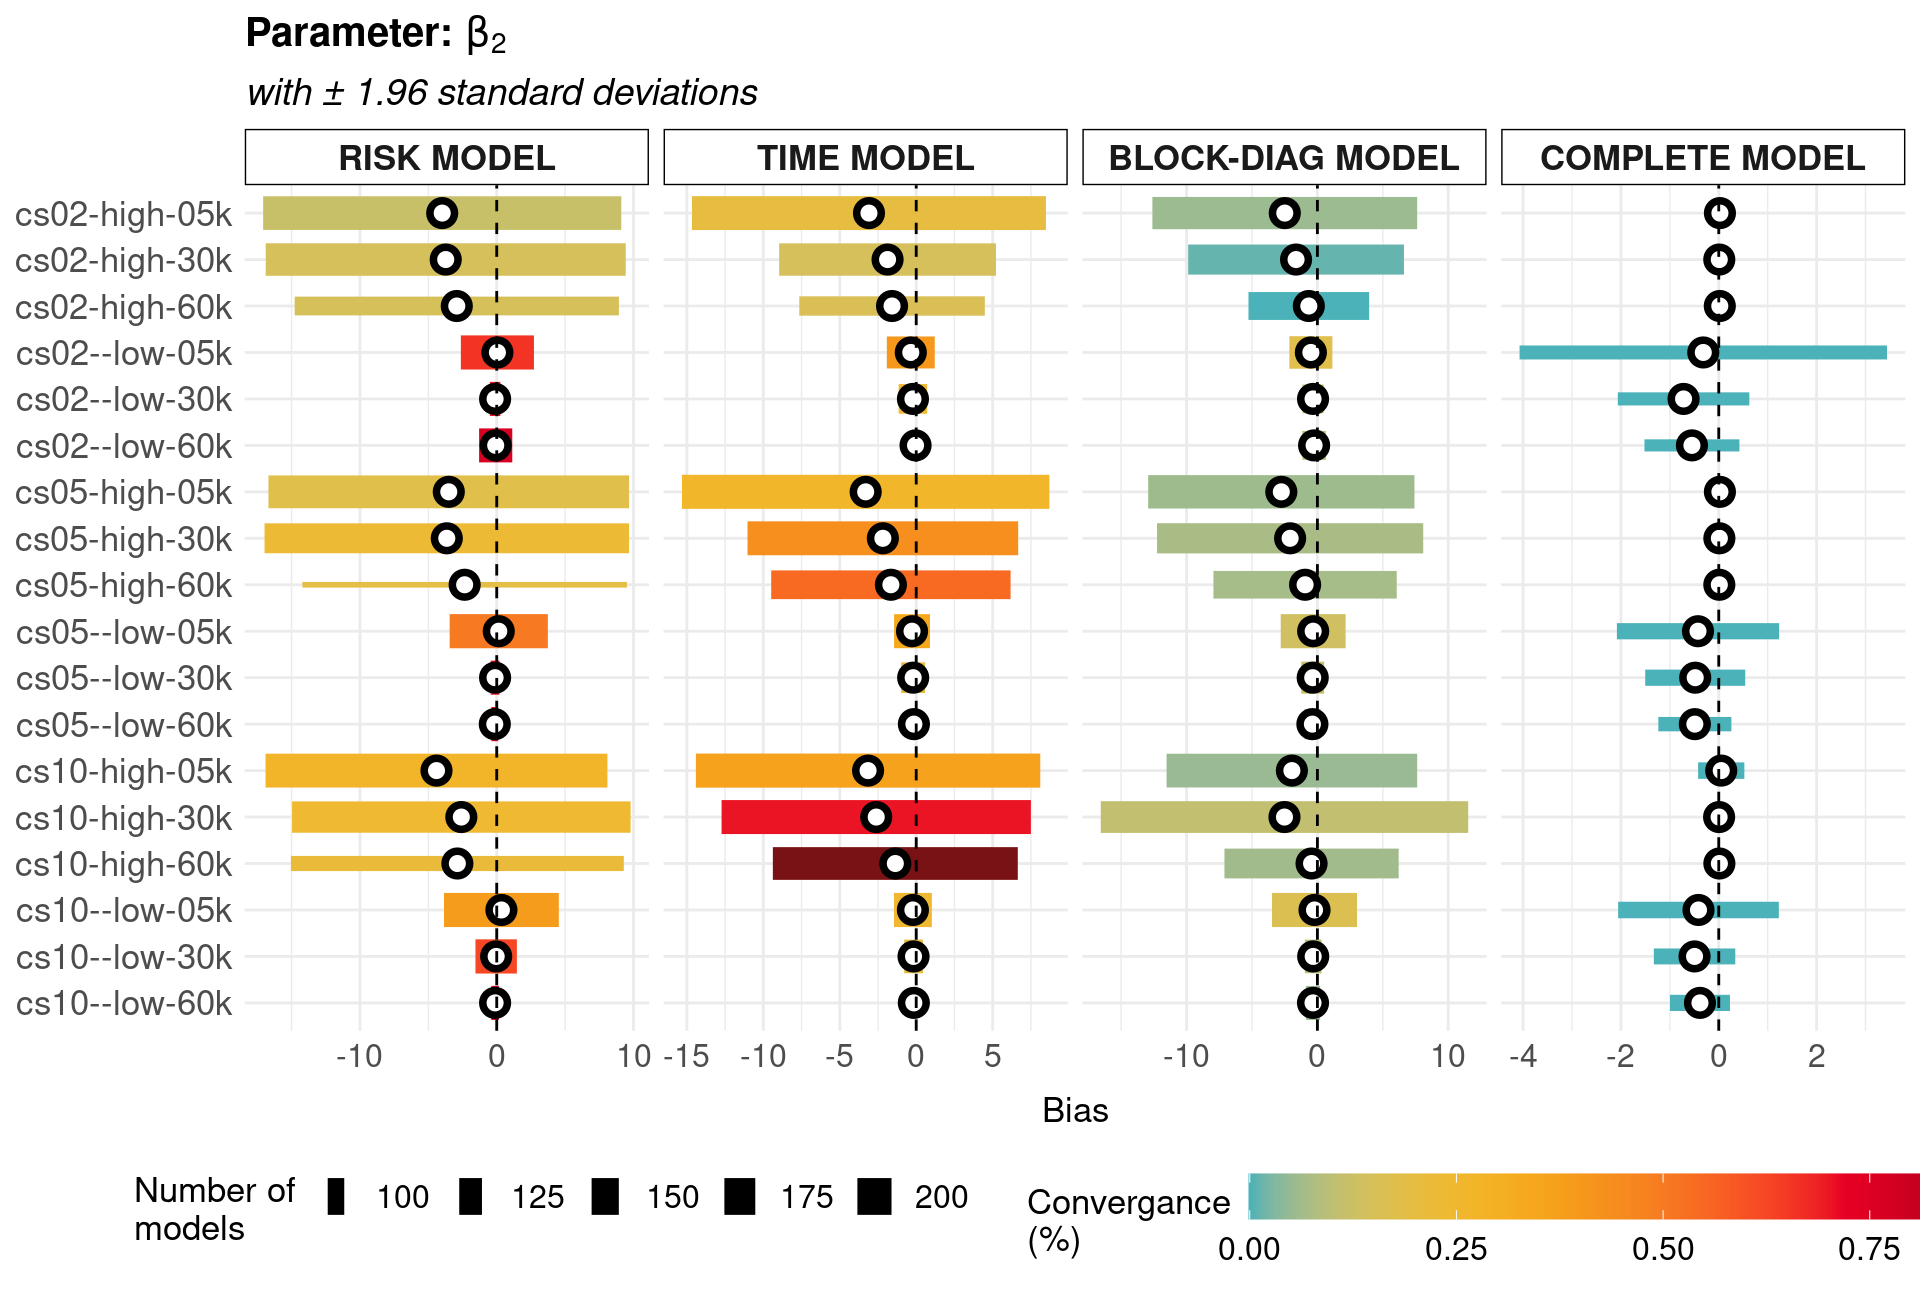
\includegraphics[width=\textwidth]{bias2plotsd-2.png}\\
 \begin{footnotesize}
  SOURCE: The author (2021).
 \end{footnotesize}
 \label{fig:biassdbeta2}
\end{figure}

\begin{figure}[H]
 \setlength{\abovecaptionskip}{.0001pt}
 \caption{PARAMETER \(\gamma_{1}\) BIAS WITH \(\pm\) 1.96 STANDARD
          DEVIATIONS}
 \vspace{0.2cm}\centering
 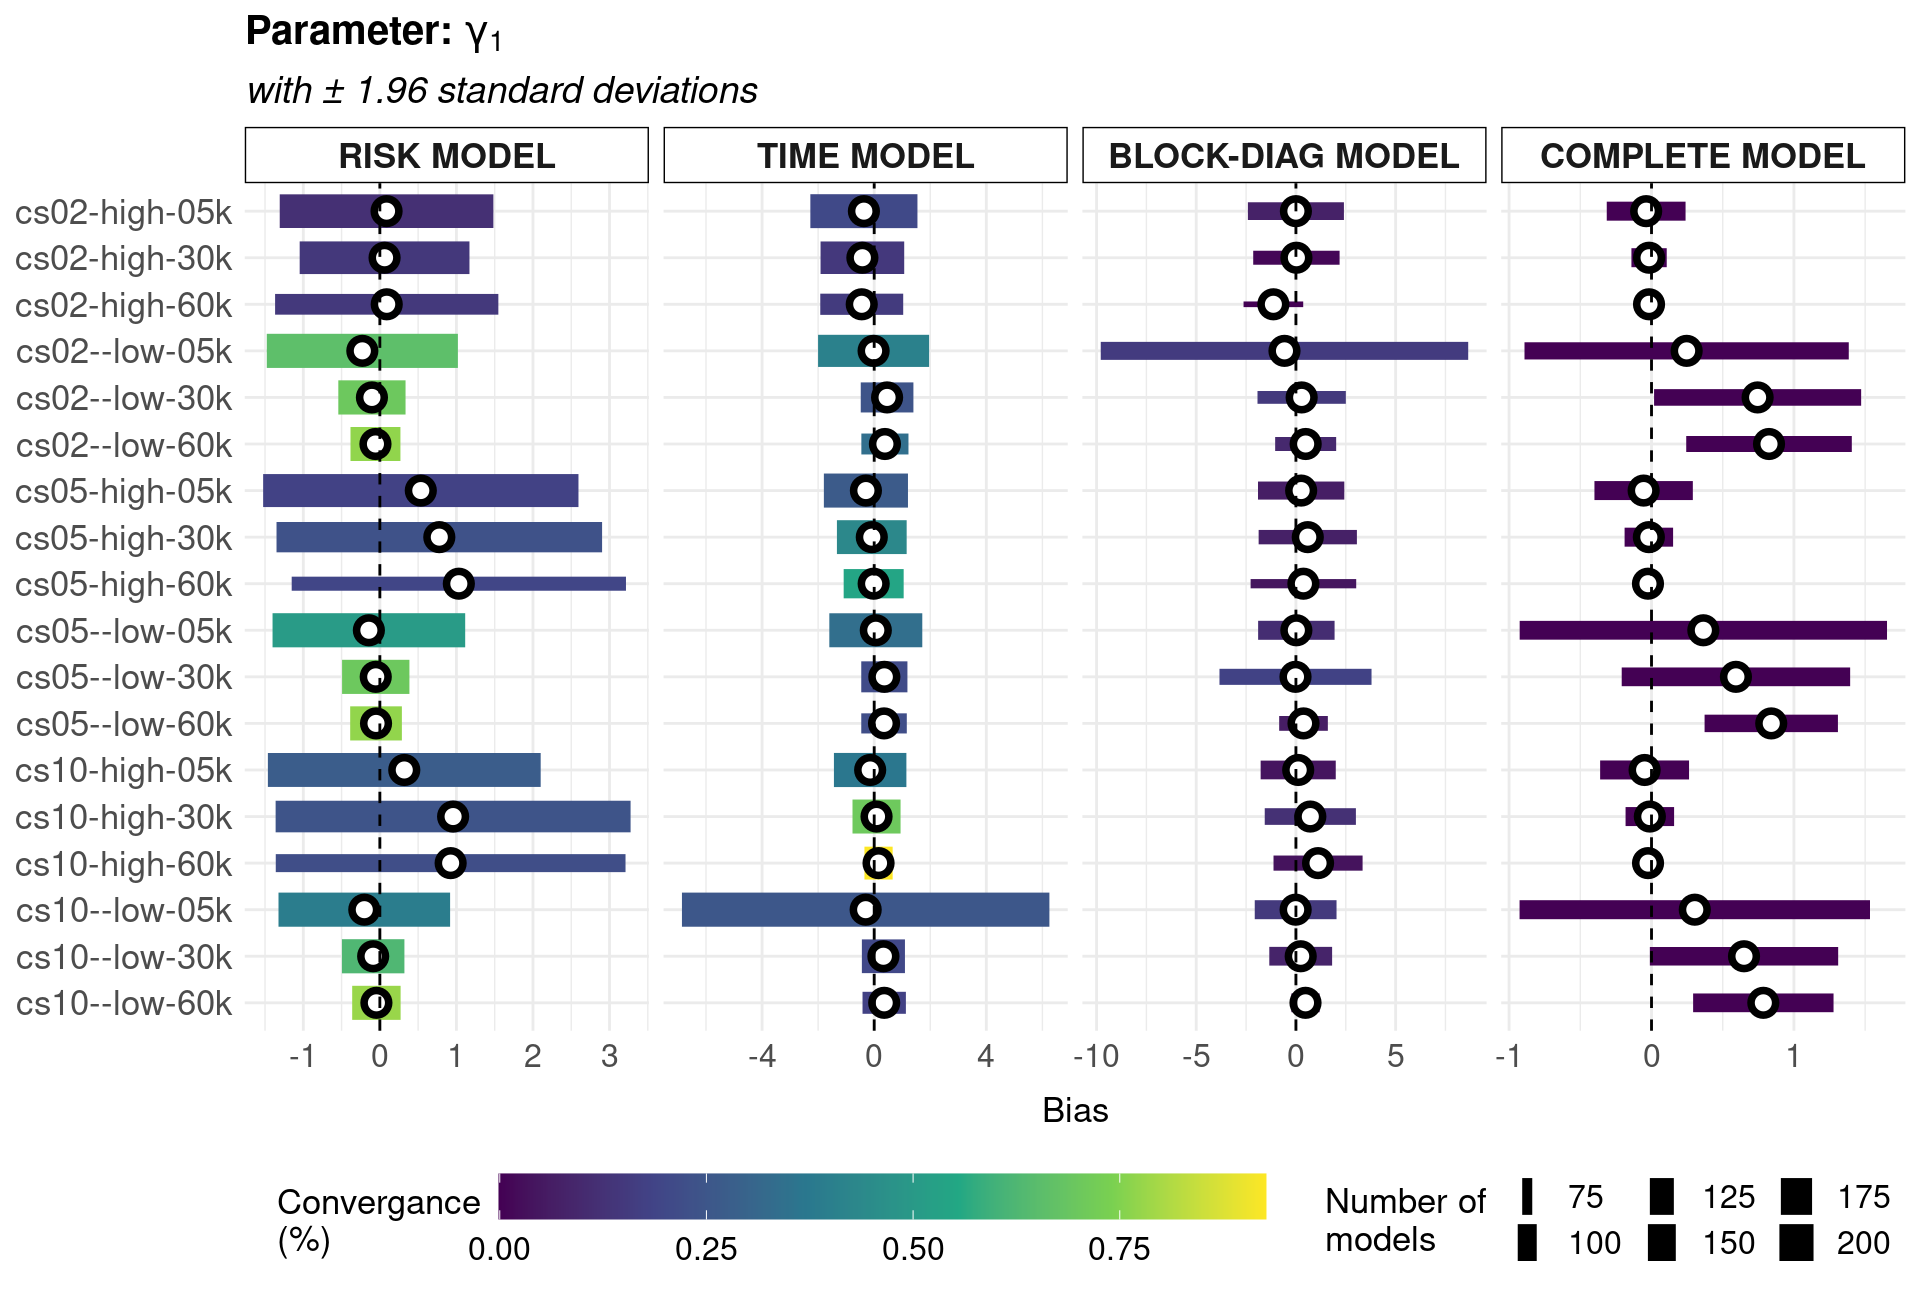
\includegraphics[width=\textwidth]{bias2plotsd-3.png}\\
 \begin{footnotesize}
  SOURCE: The author (2021).
 \end{footnotesize}
 \label{fig:biassdgama1}
\end{figure}

\begin{figure}[H]
 \setlength{\abovecaptionskip}{.0001pt}
 \caption{PARAMETER \(\gamma_{2}\) BIAS WITH \(\pm\) 1.96 STANDARD
          DEVIATIONS}
 \vspace{0.2cm}\centering
 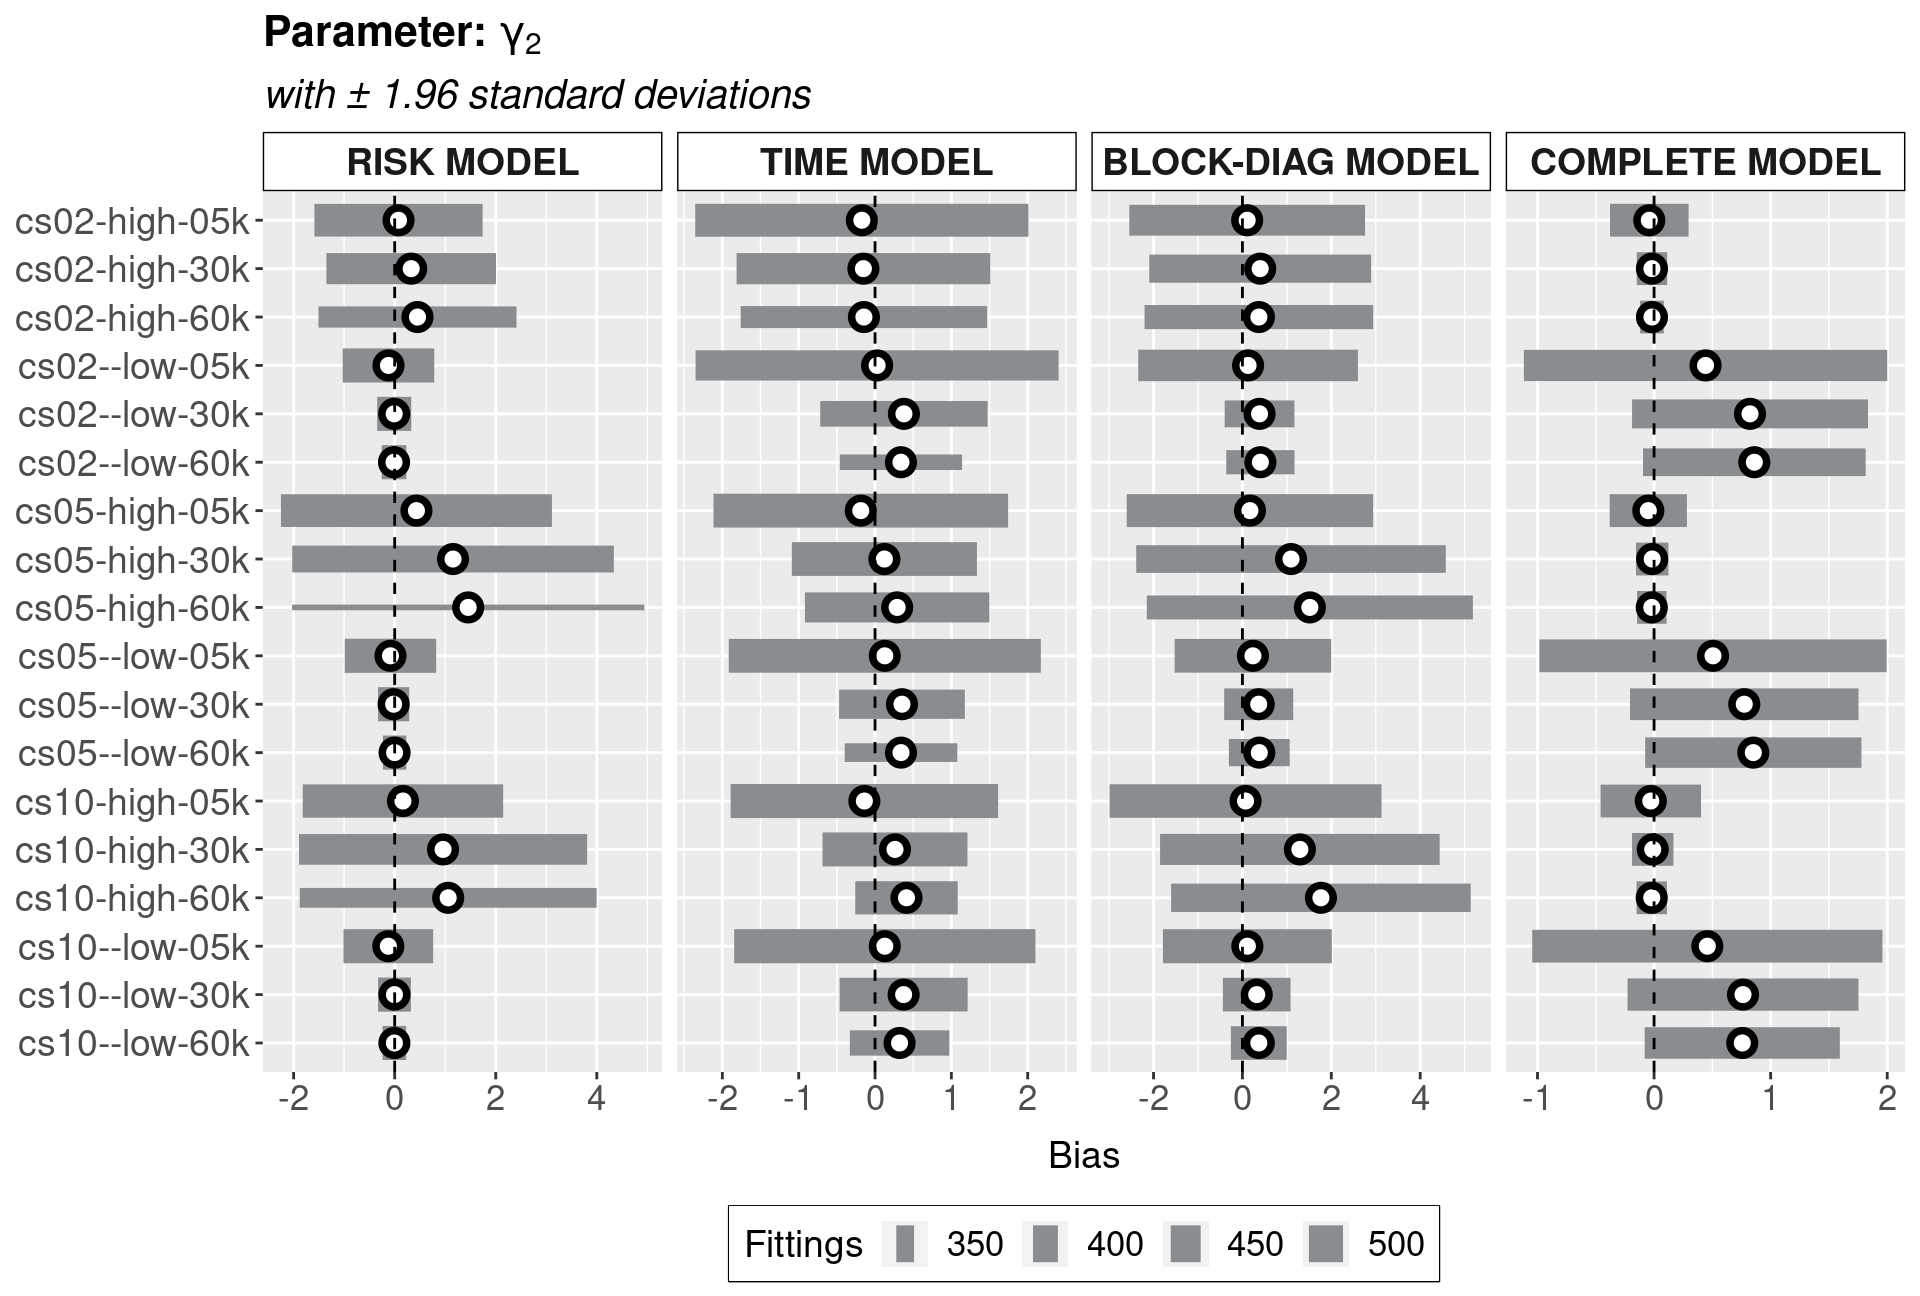
\includegraphics[width=\textwidth]{bias2plotsd-4.png}\\
 \begin{footnotesize}
  SOURCE: The author (2021).
 \end{footnotesize}
 \label{fig:biassdgama2}
\end{figure}

\begin{figure}[H]
 \setlength{\abovecaptionskip}{.0001pt}
 \caption{PARAMETER \(w_{1}\) BIAS WITH \(\pm\) 1.96 STANDARD DEVIATIONS}
 \vspace{0.2cm}\centering
 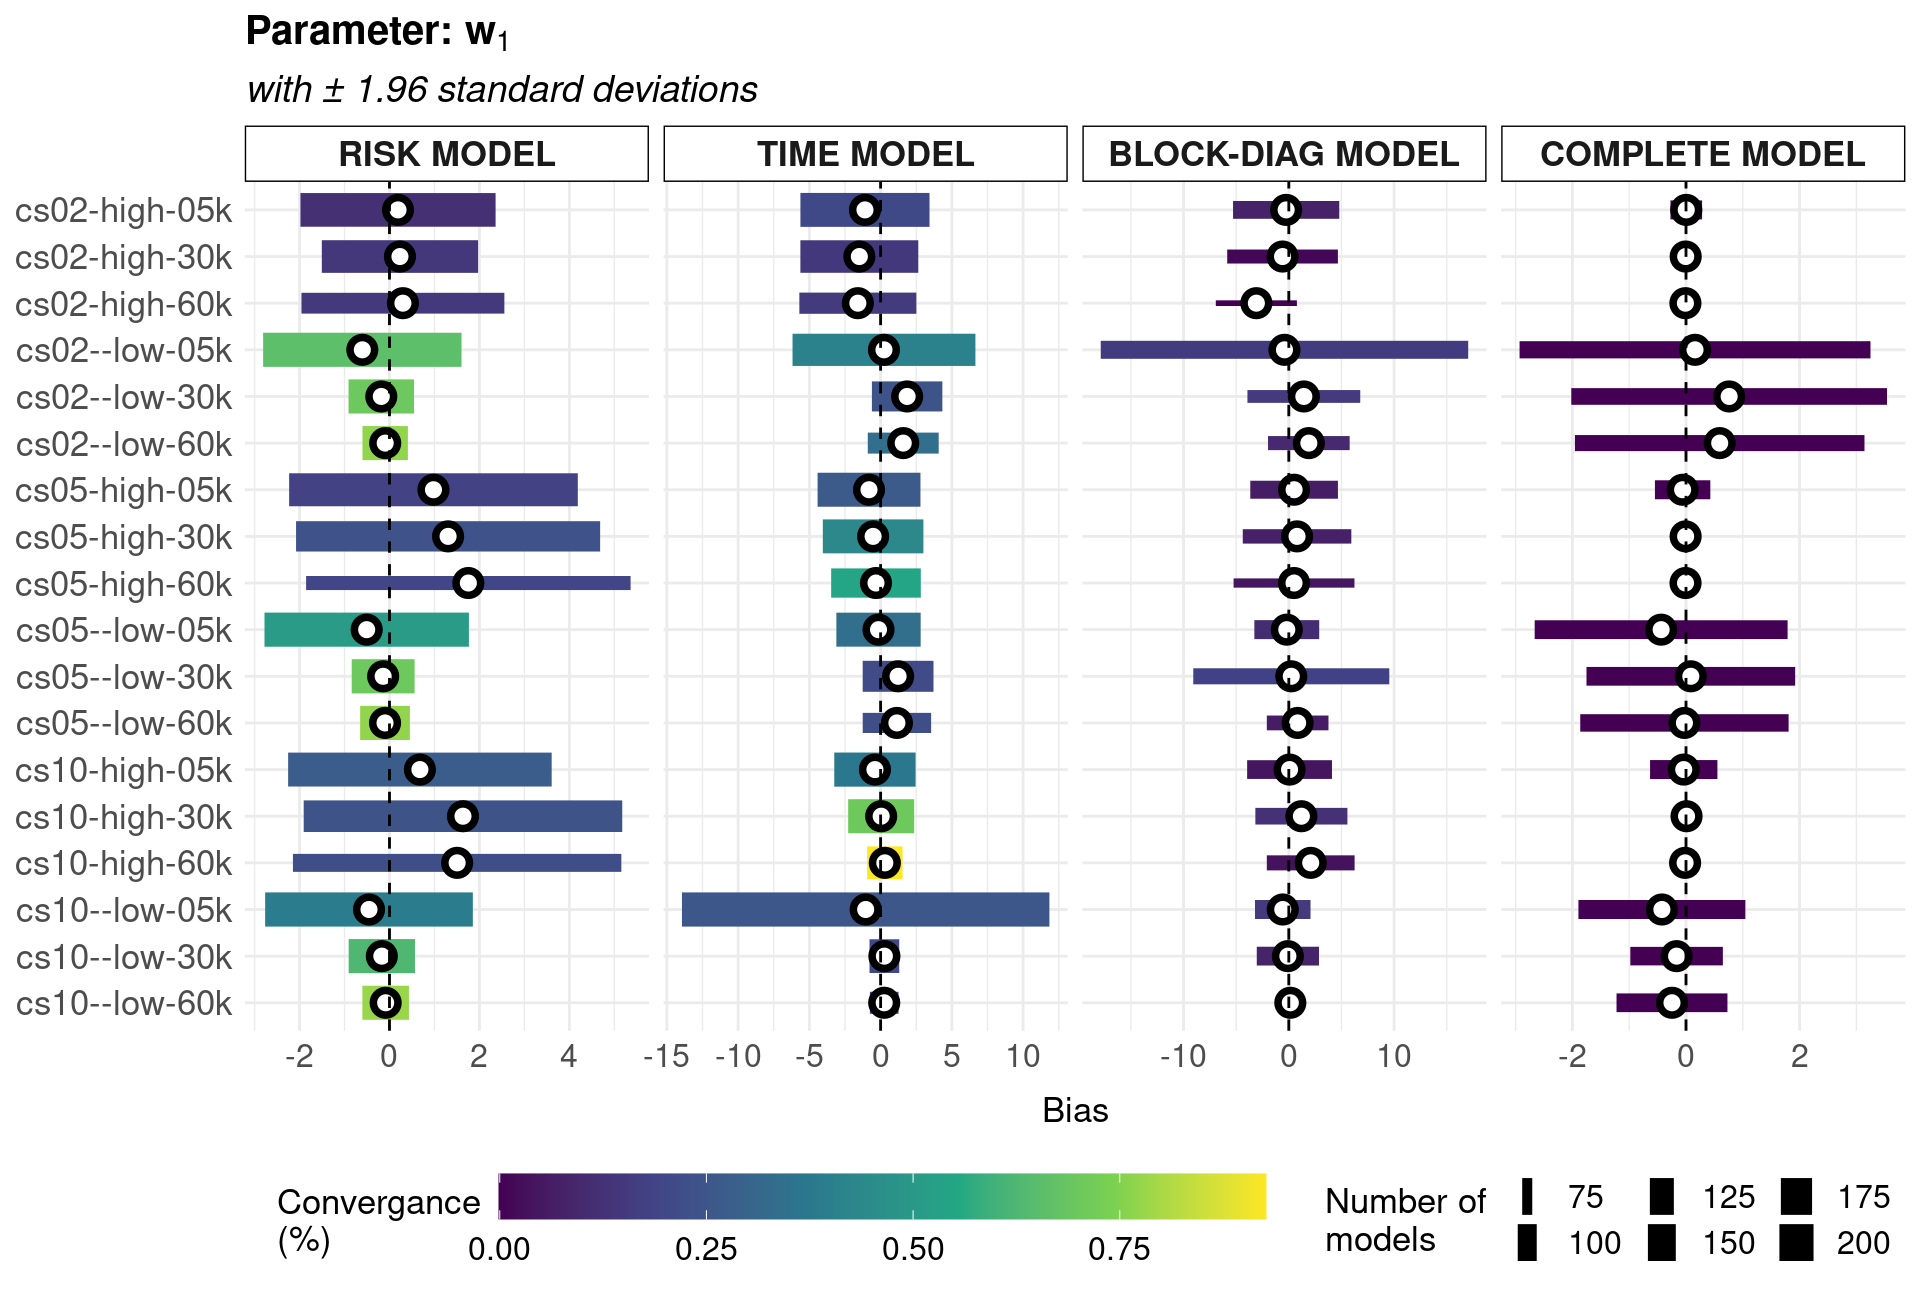
\includegraphics[width=\textwidth]{bias2plotsd-5.png}\\
 \begin{footnotesize}
  SOURCE: The author (2021).
 \end{footnotesize}
 \label{fig:biassdw1}
\end{figure}

\begin{figure}[H]
 \setlength{\abovecaptionskip}{.0001pt}
 \caption{PARAMETER \(w_{2}\) BIAS WITH \(\pm\) 1.96 STANDARD DEVIATIONS}
 \vspace{0.2cm}\centering
 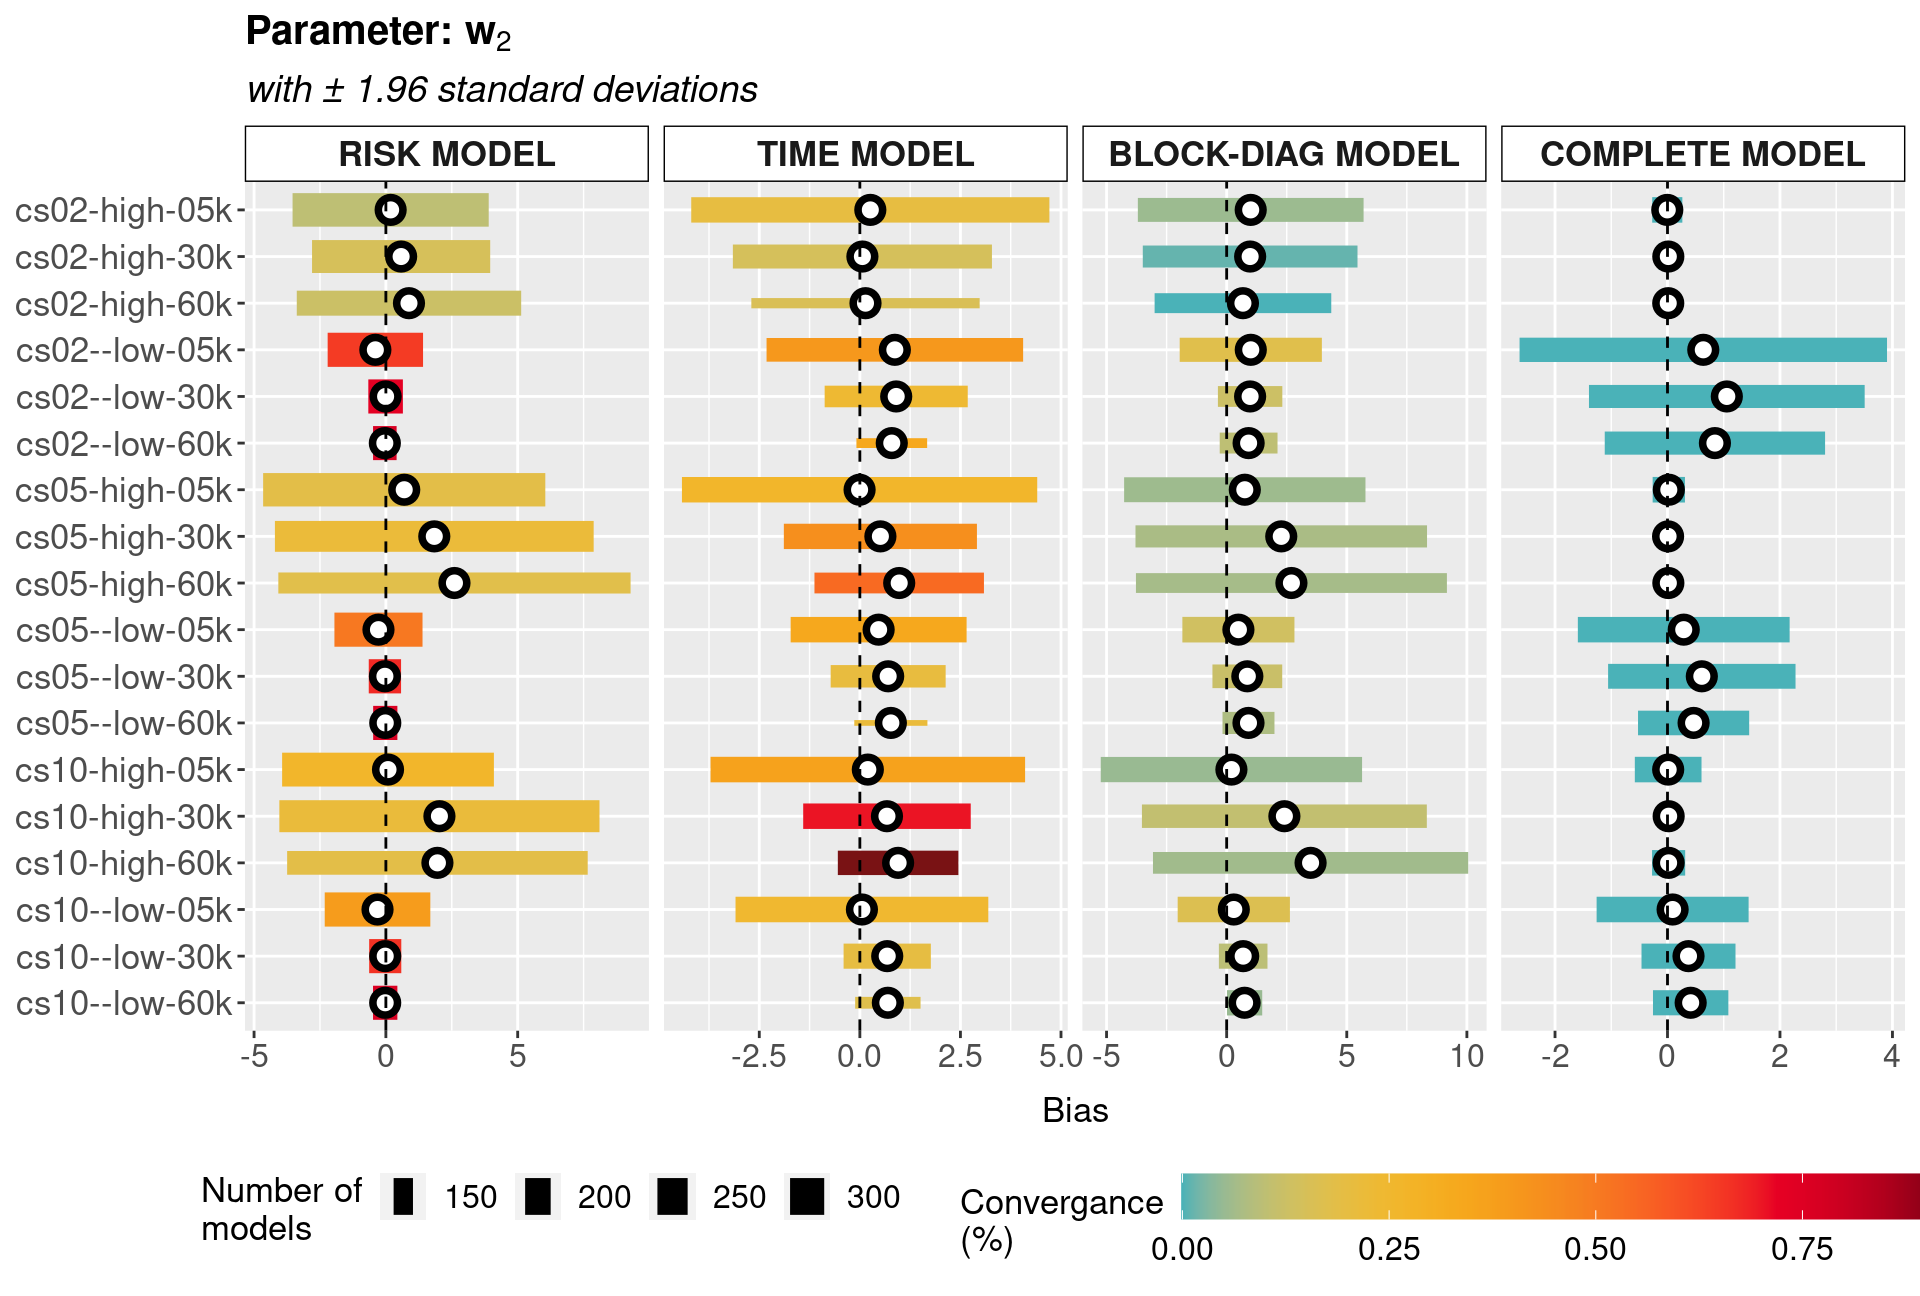
\includegraphics[width=\textwidth]{bias2plotsd-6.png}\\
 \begin{footnotesize}
  SOURCE: The author (2021).
 \end{footnotesize}
 \label{fig:biassdw2}
\end{figure}

\begin{figure}[H]
 \setlength{\abovecaptionskip}{.0001pt}
 \caption{PARAMETER \(\log(\sigma_{1}^{2})\) BIAS WITH \(\pm\) 1.96
          STANDARD DEVIATIONS}
 \vspace{0.2cm}\centering
 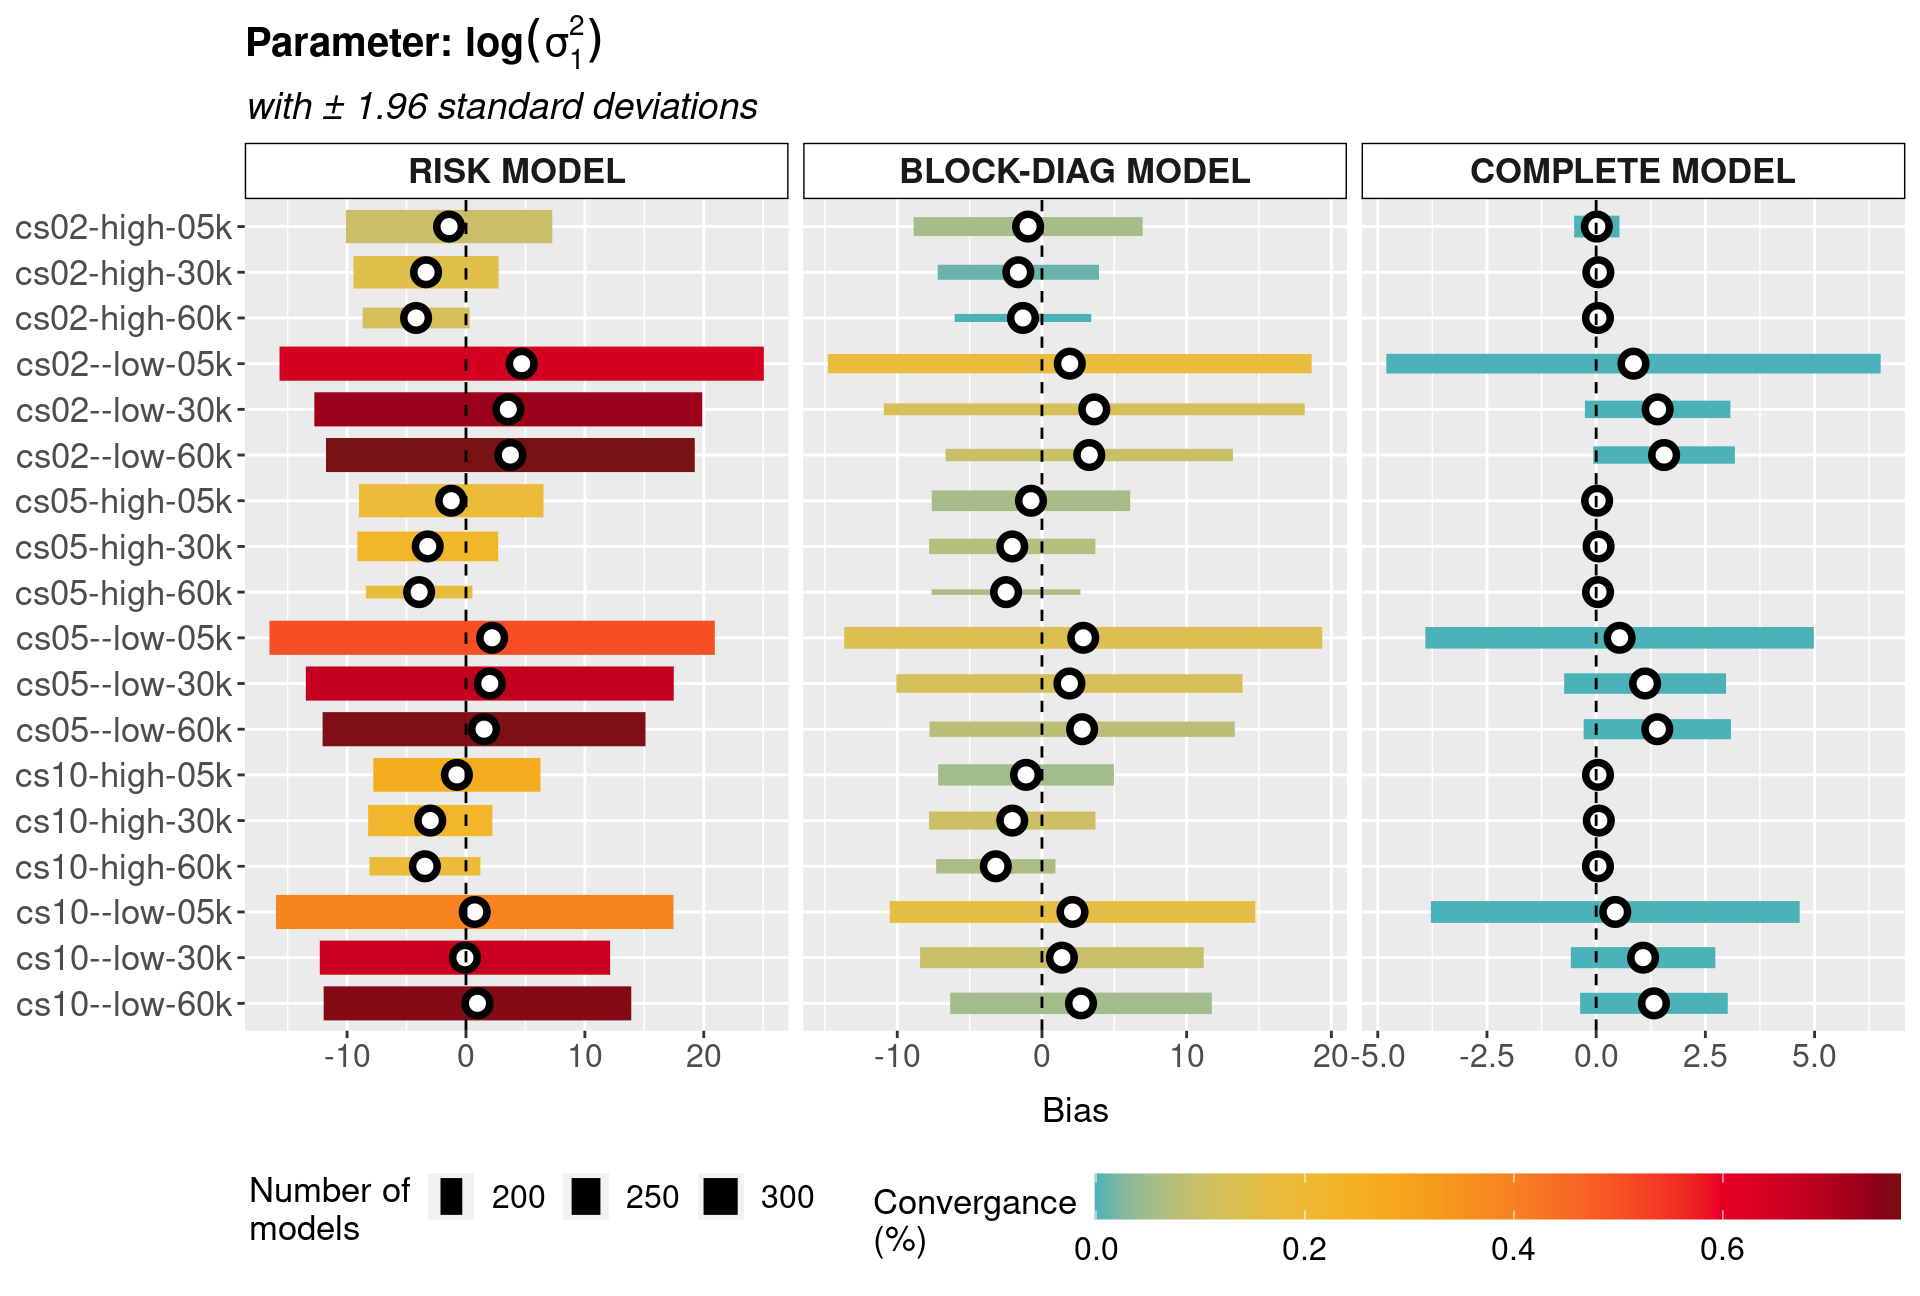
\includegraphics[width=\textwidth]{bias2plotsd-7.png}\\
 \begin{footnotesize}
  SOURCE: The author (2021).
 \end{footnotesize}
 \label{fig:biassdlogs2_1}
\end{figure}

\begin{figure}[H]
 \setlength{\abovecaptionskip}{.0001pt}
 \caption{PARAMETER \(\log(\sigma_{2}^{2})\) BIAS WITH \(\pm\) 1.96
          STANDARD DEVIATIONS}
 \vspace{0.2cm}\centering
 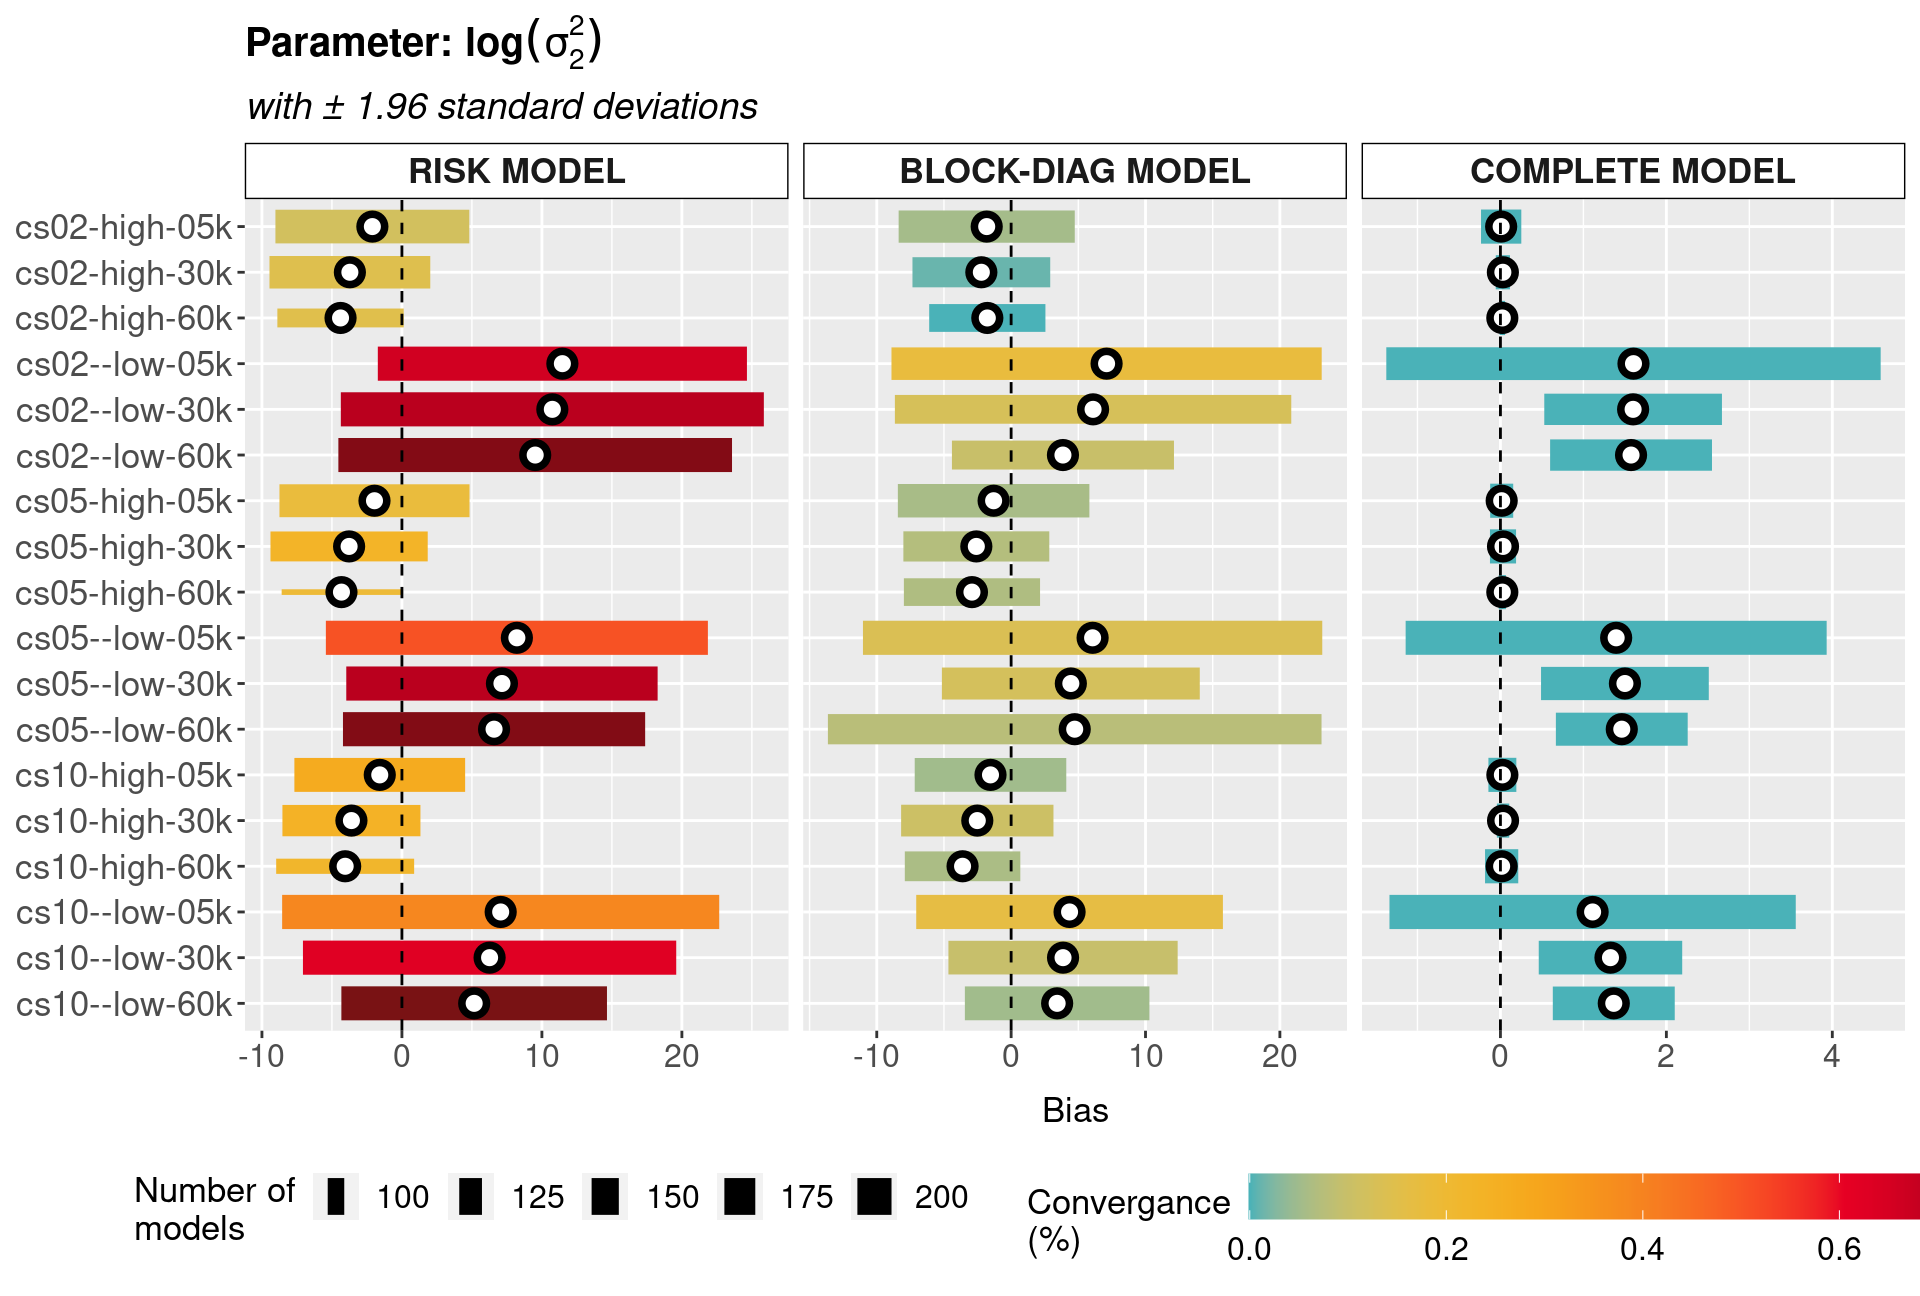
\includegraphics[width=\textwidth]{bias2plotsd-8.png}\\
 \begin{footnotesize}
  SOURCE: The author (2021).
 \end{footnotesize}
 \label{fig:biassdlogs2_2}
\end{figure}

\begin{figure}[H]
 \setlength{\abovecaptionskip}{.0001pt}
 \caption{PARAMETER \(\log(\sigma_{3}^{2})\) BIAS WITH \(\pm\) 1.96
          STANDARD DEVIATIONS}
 \vspace{0.2cm}\centering
 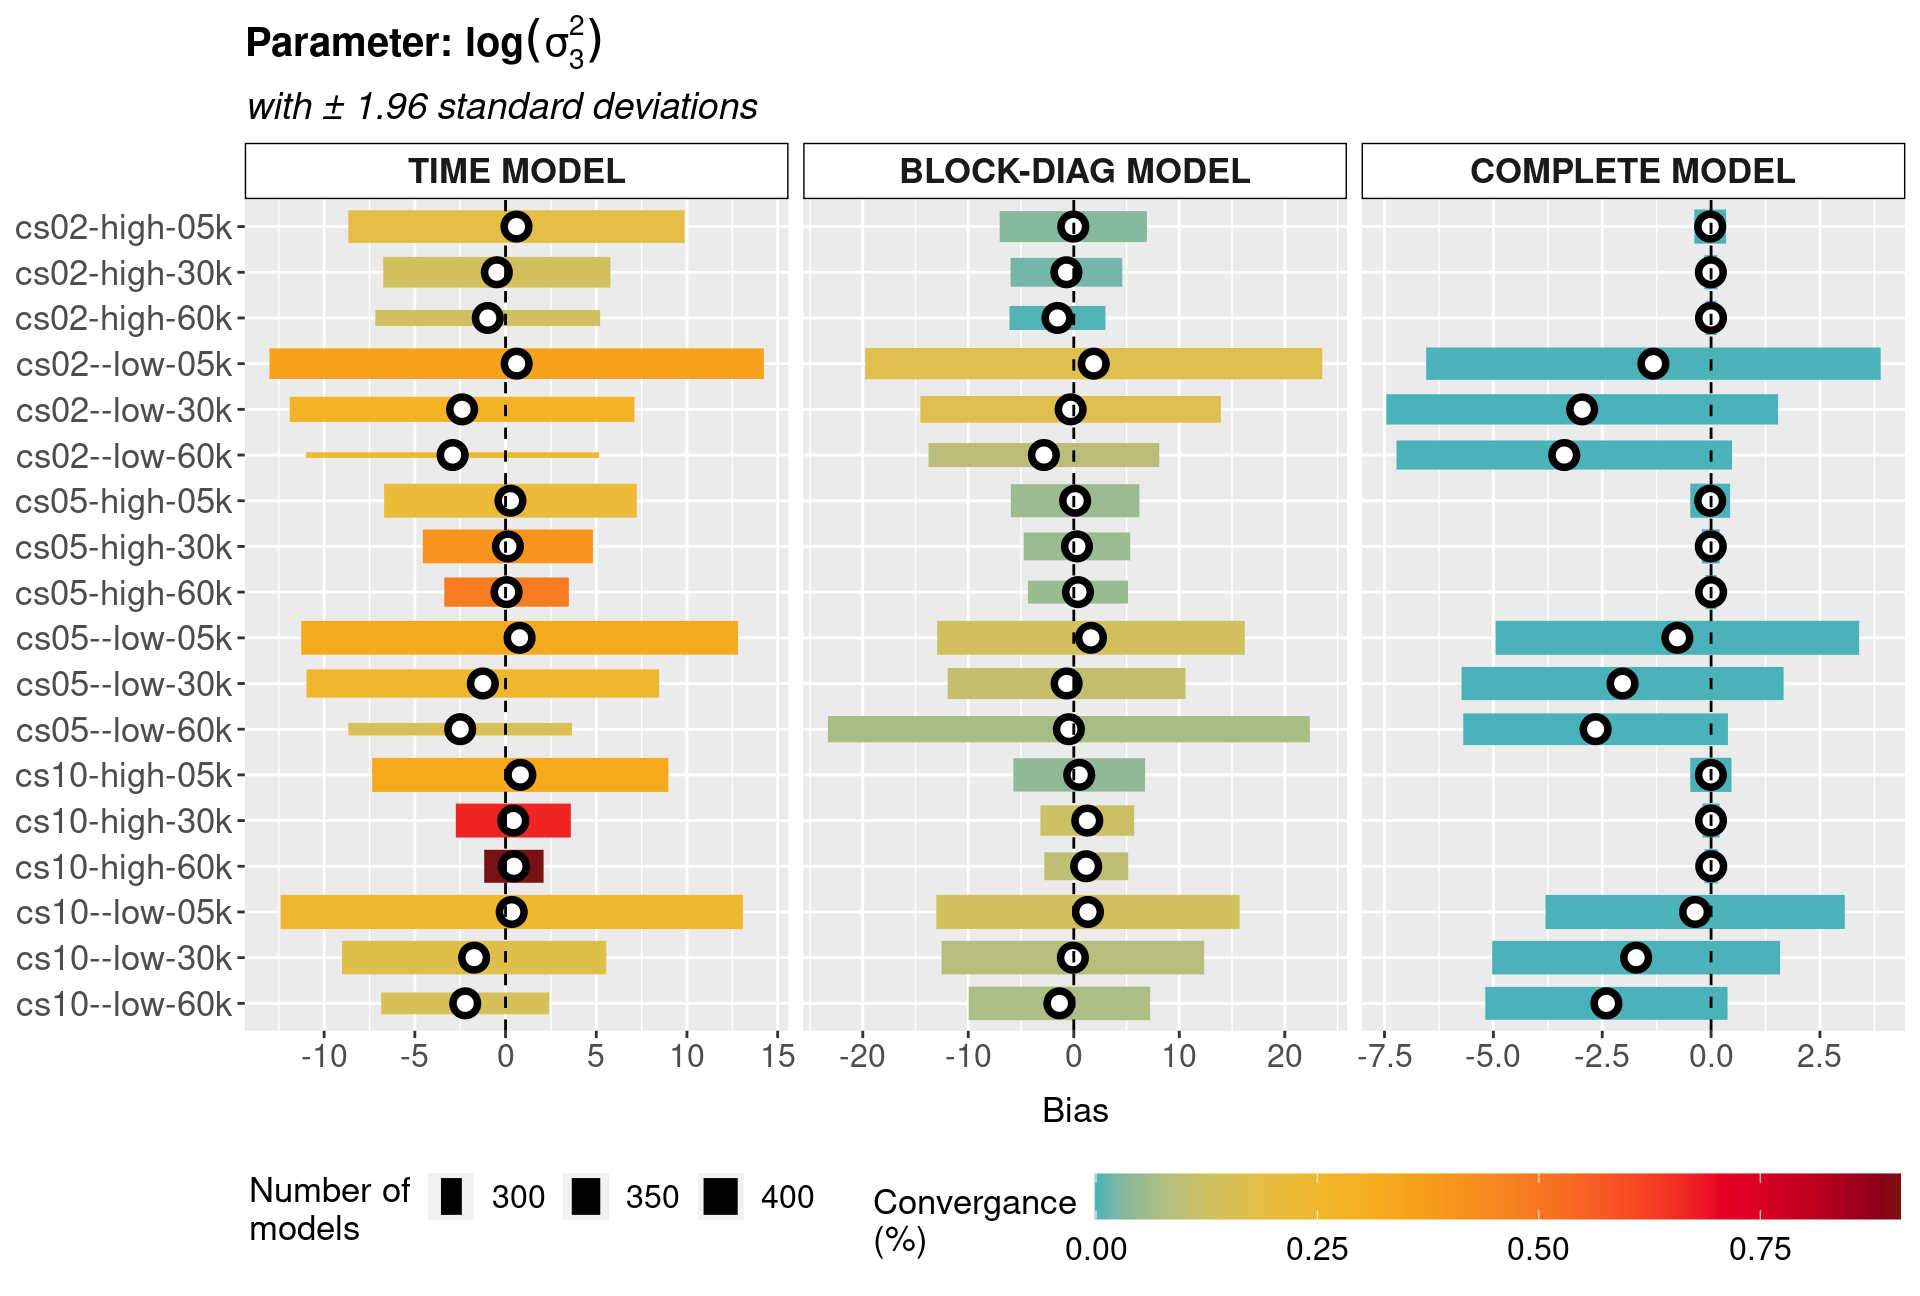
\includegraphics[width=\textwidth]{bias2plotsd-9.png}\\
 \begin{footnotesize}
  SOURCE: The author (2021).
 \end{footnotesize}
 \label{fig:biassdlogs2_3}
\end{figure}

\begin{figure}[H]
 \setlength{\abovecaptionskip}{.0001pt}
 \caption{PARAMETER \(\log(\sigma_{4}^{2})\) BIAS WITH \(\pm\) 1.96
          STANDARD DEVIATIONS}
 \vspace{0.2cm}\centering
 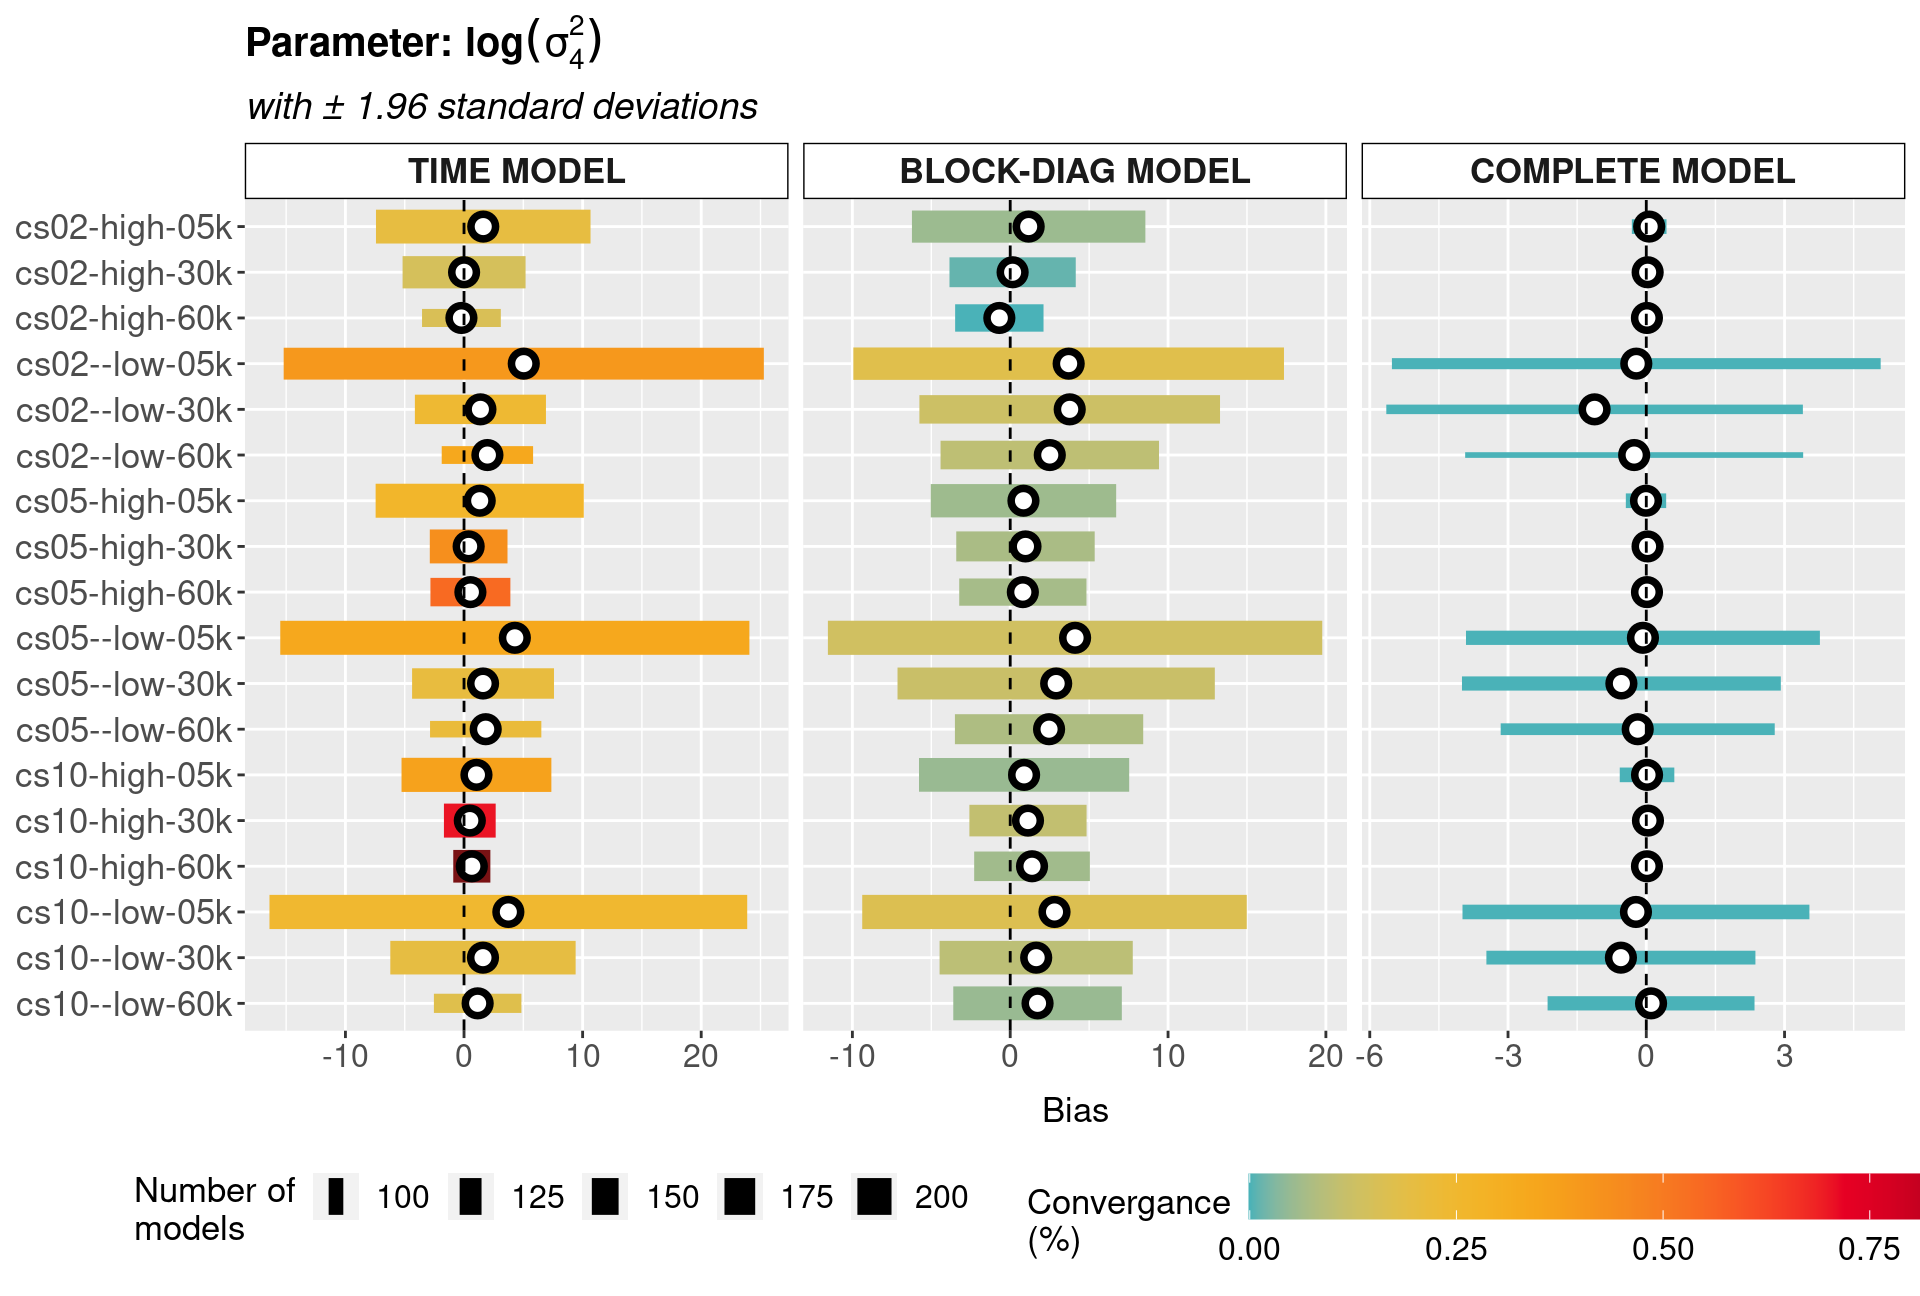
\includegraphics[width=\textwidth]{bias2plotsd-10.png}\\
 \begin{footnotesize}
  SOURCE: The author (2021).
 \end{footnotesize}
 \label{fig:biassdlogs2_4}
\end{figure}

\begin{figure}[H]
 \setlength{\abovecaptionskip}{.0001pt}
 \caption{PARAMETER \(z(\rho_{12})\) BIAS WITH \(\pm\) 1.96 STANDARD
          DEVIATIONS}
 \vspace{0.2cm}\centering
 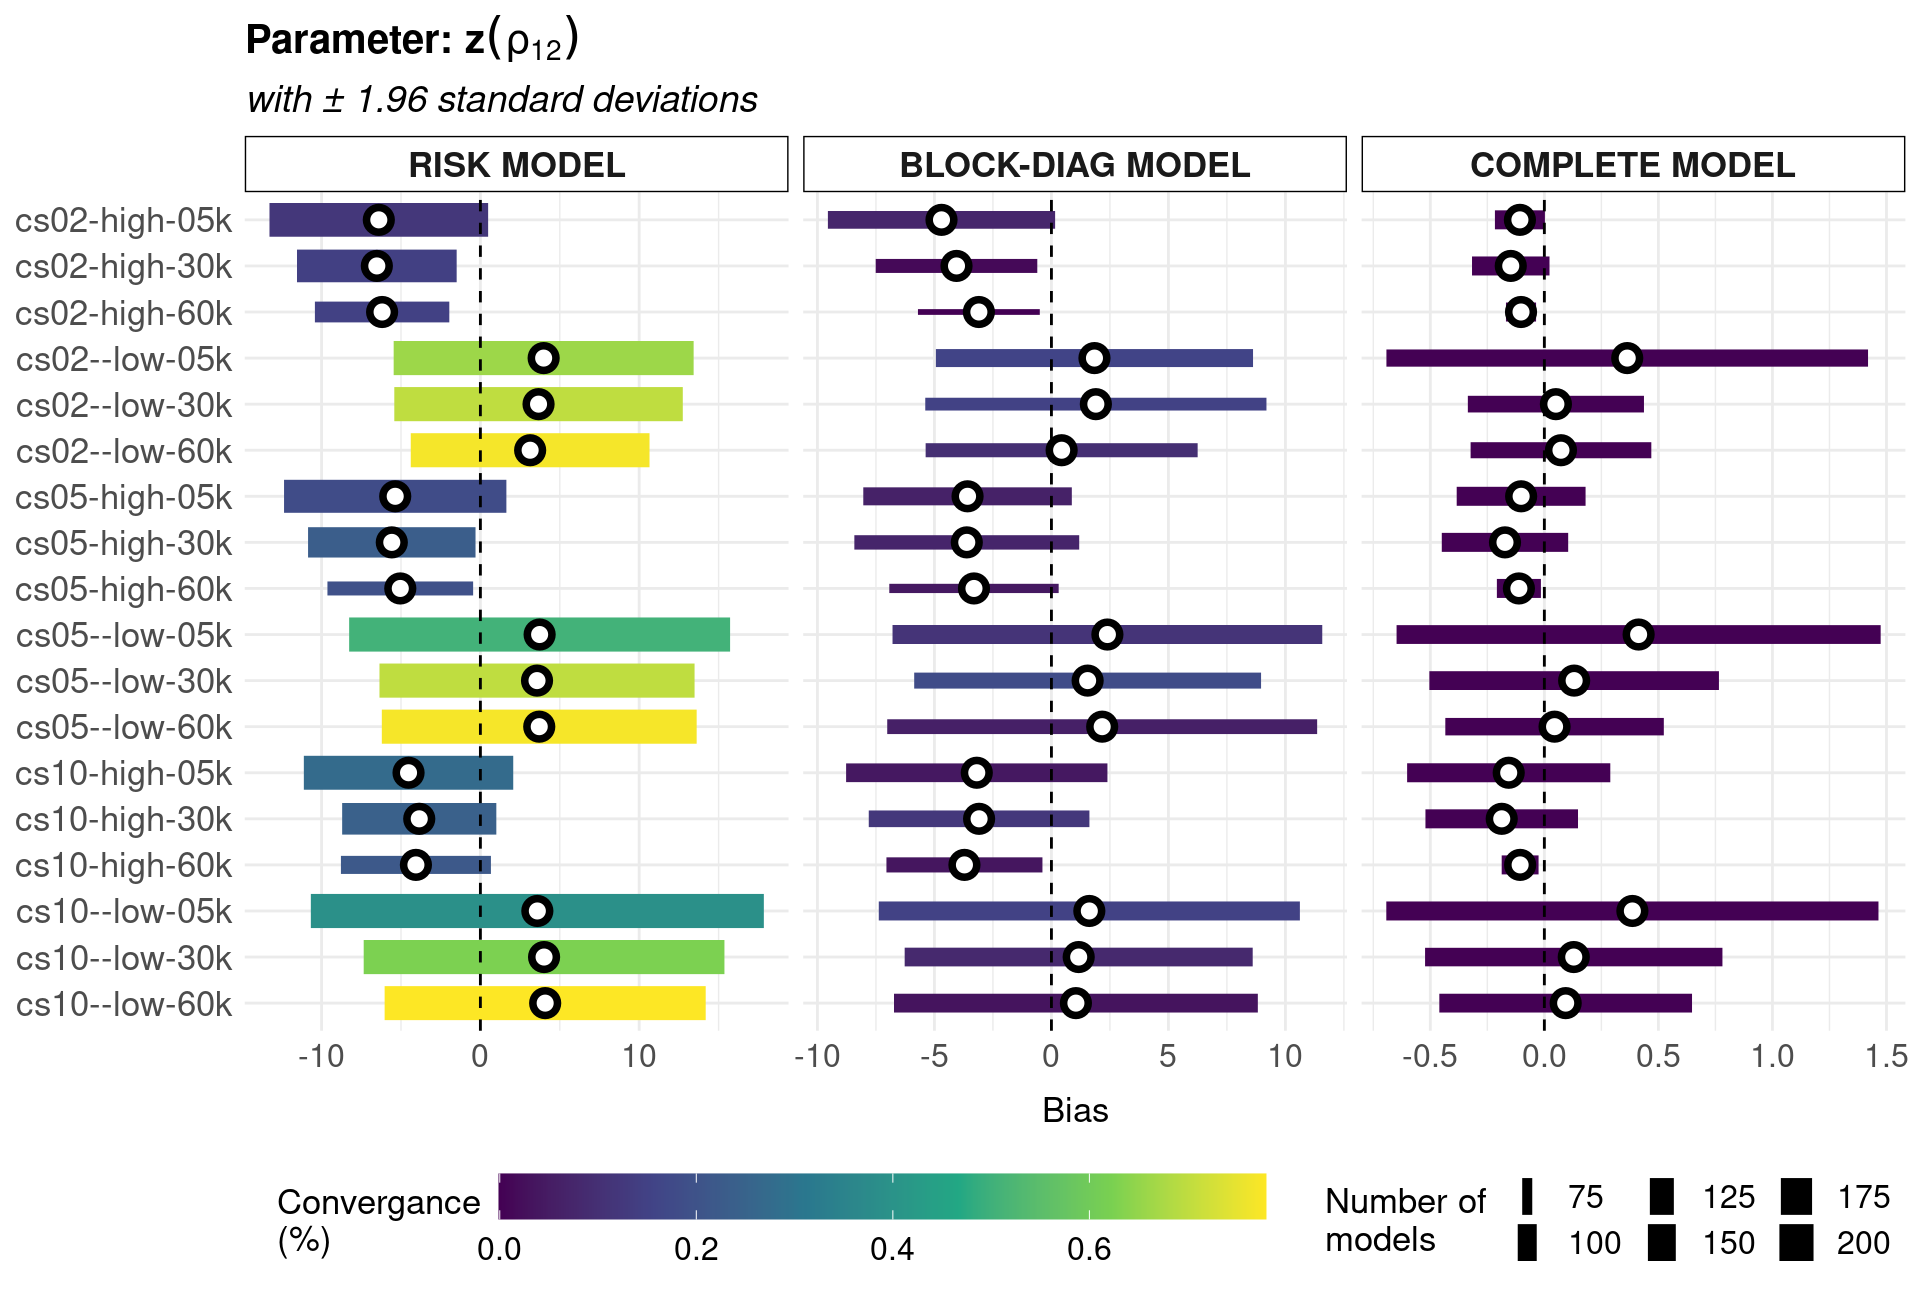
\includegraphics[width=\textwidth]{bias2plotsd-11.png}\\
 \begin{footnotesize}
  SOURCE: The author (2021).
 \end{footnotesize}
 \label{fig:biassdrhoz12}
\end{figure}

\begin{figure}[H]
 \setlength{\abovecaptionskip}{.0001pt}
 \caption{PARAMETER \(z(\rho_{34})\) BIAS WITH \(\pm\) 1.96 STANDARD
          DEVIATIONS}
 \vspace{0.2cm}\centering
 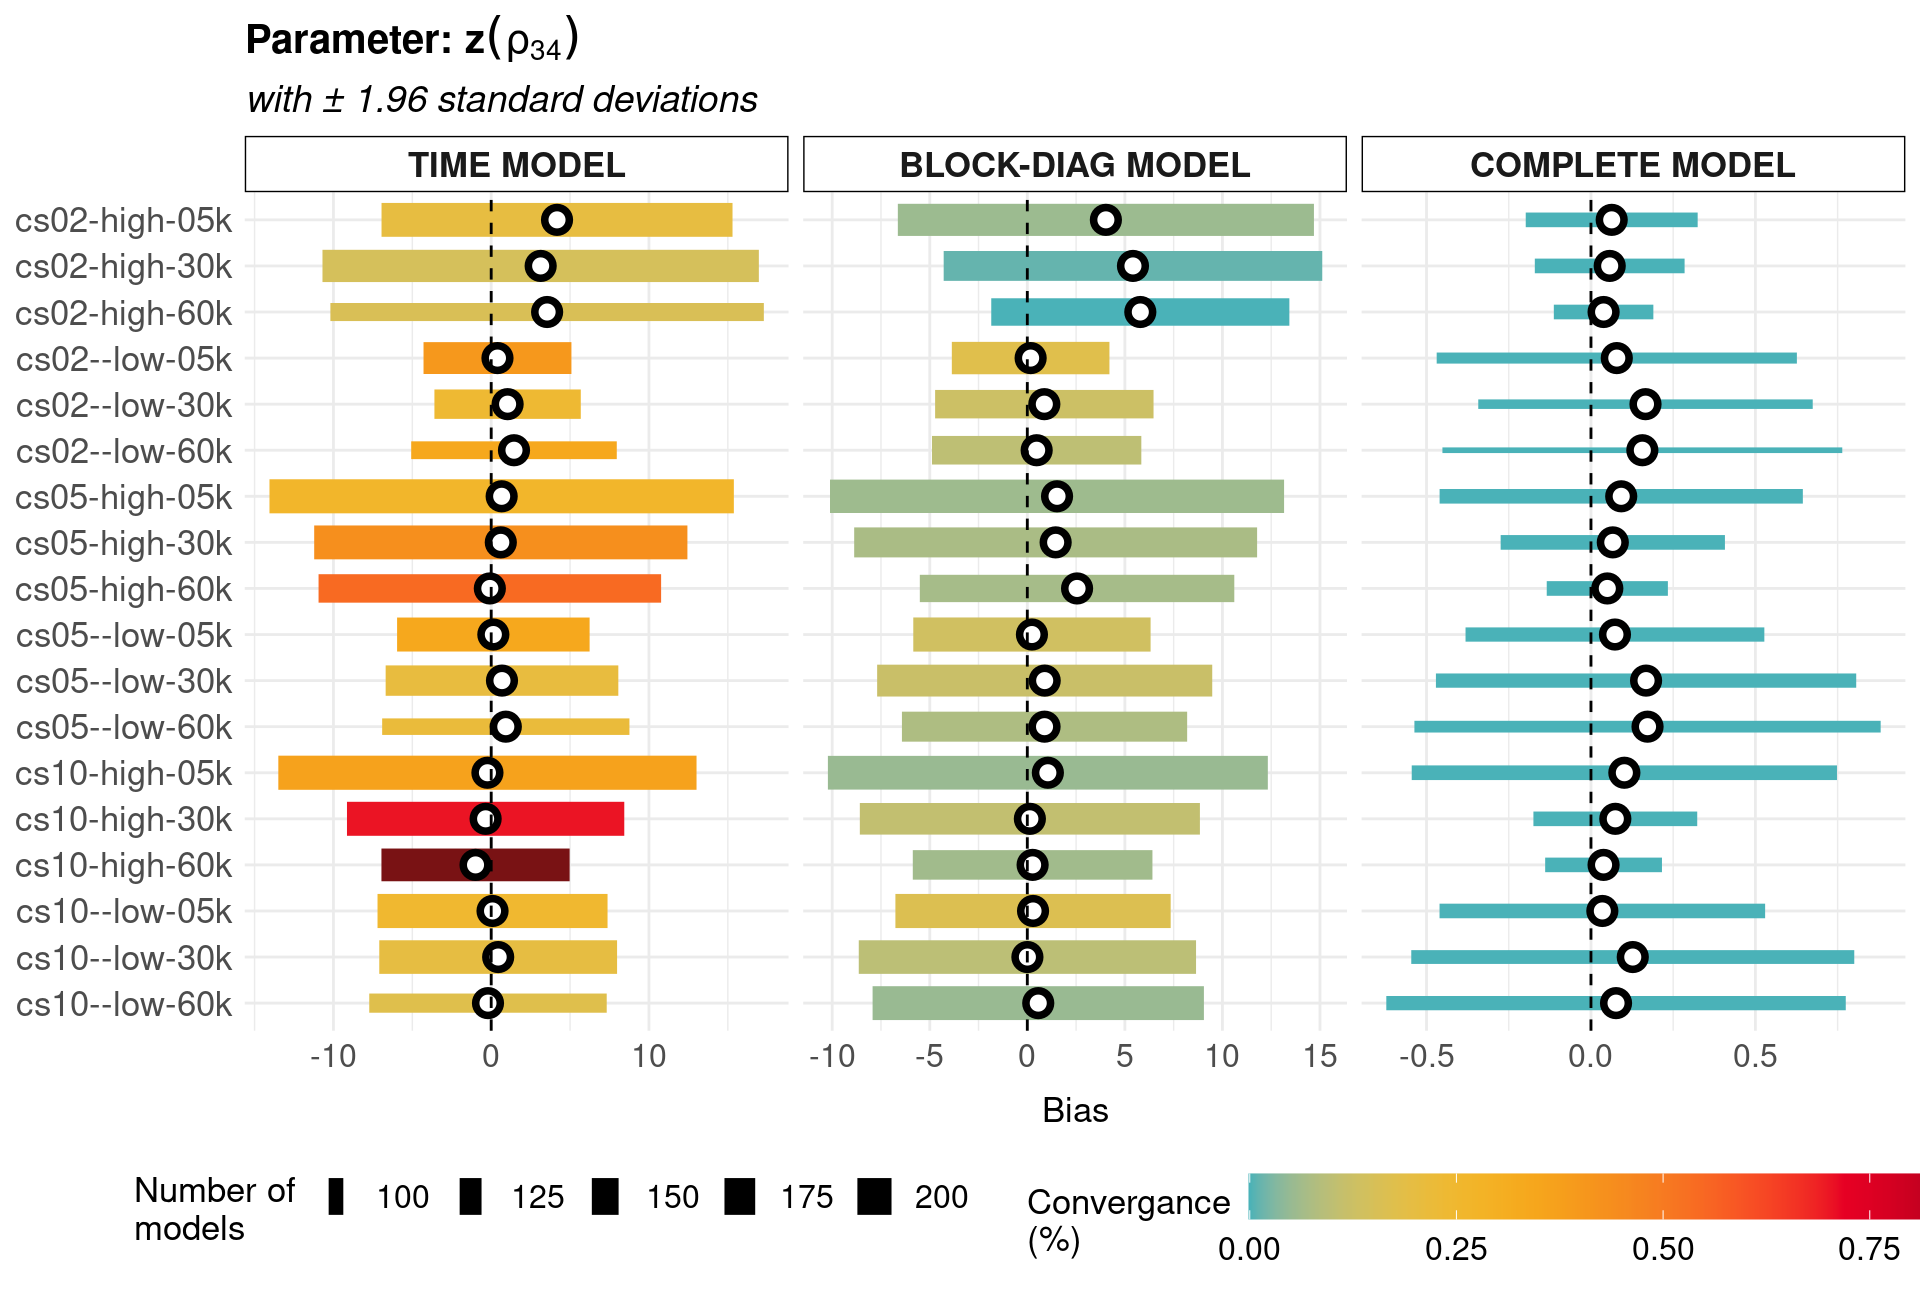
\includegraphics[width=\textwidth]{bias2plotsd-12.png}\\
 \begin{footnotesize}
  SOURCE: The author (2021).
 \end{footnotesize}
 \label{fig:biassdrhoz34}
\end{figure}

\begin{figure}[H]
 \setlength{\abovecaptionskip}{.0001pt}
 \caption{PARAMETERS
          \(\{z(\rho_{13}),~z(\rho_{24}),~z(\rho_{14}),~z(\rho_{23})\}\)
          BIAS WITH \(\pm\) 1.96 STANDARD DEVIATIONS}
 \vspace{0.2cm}\centering
 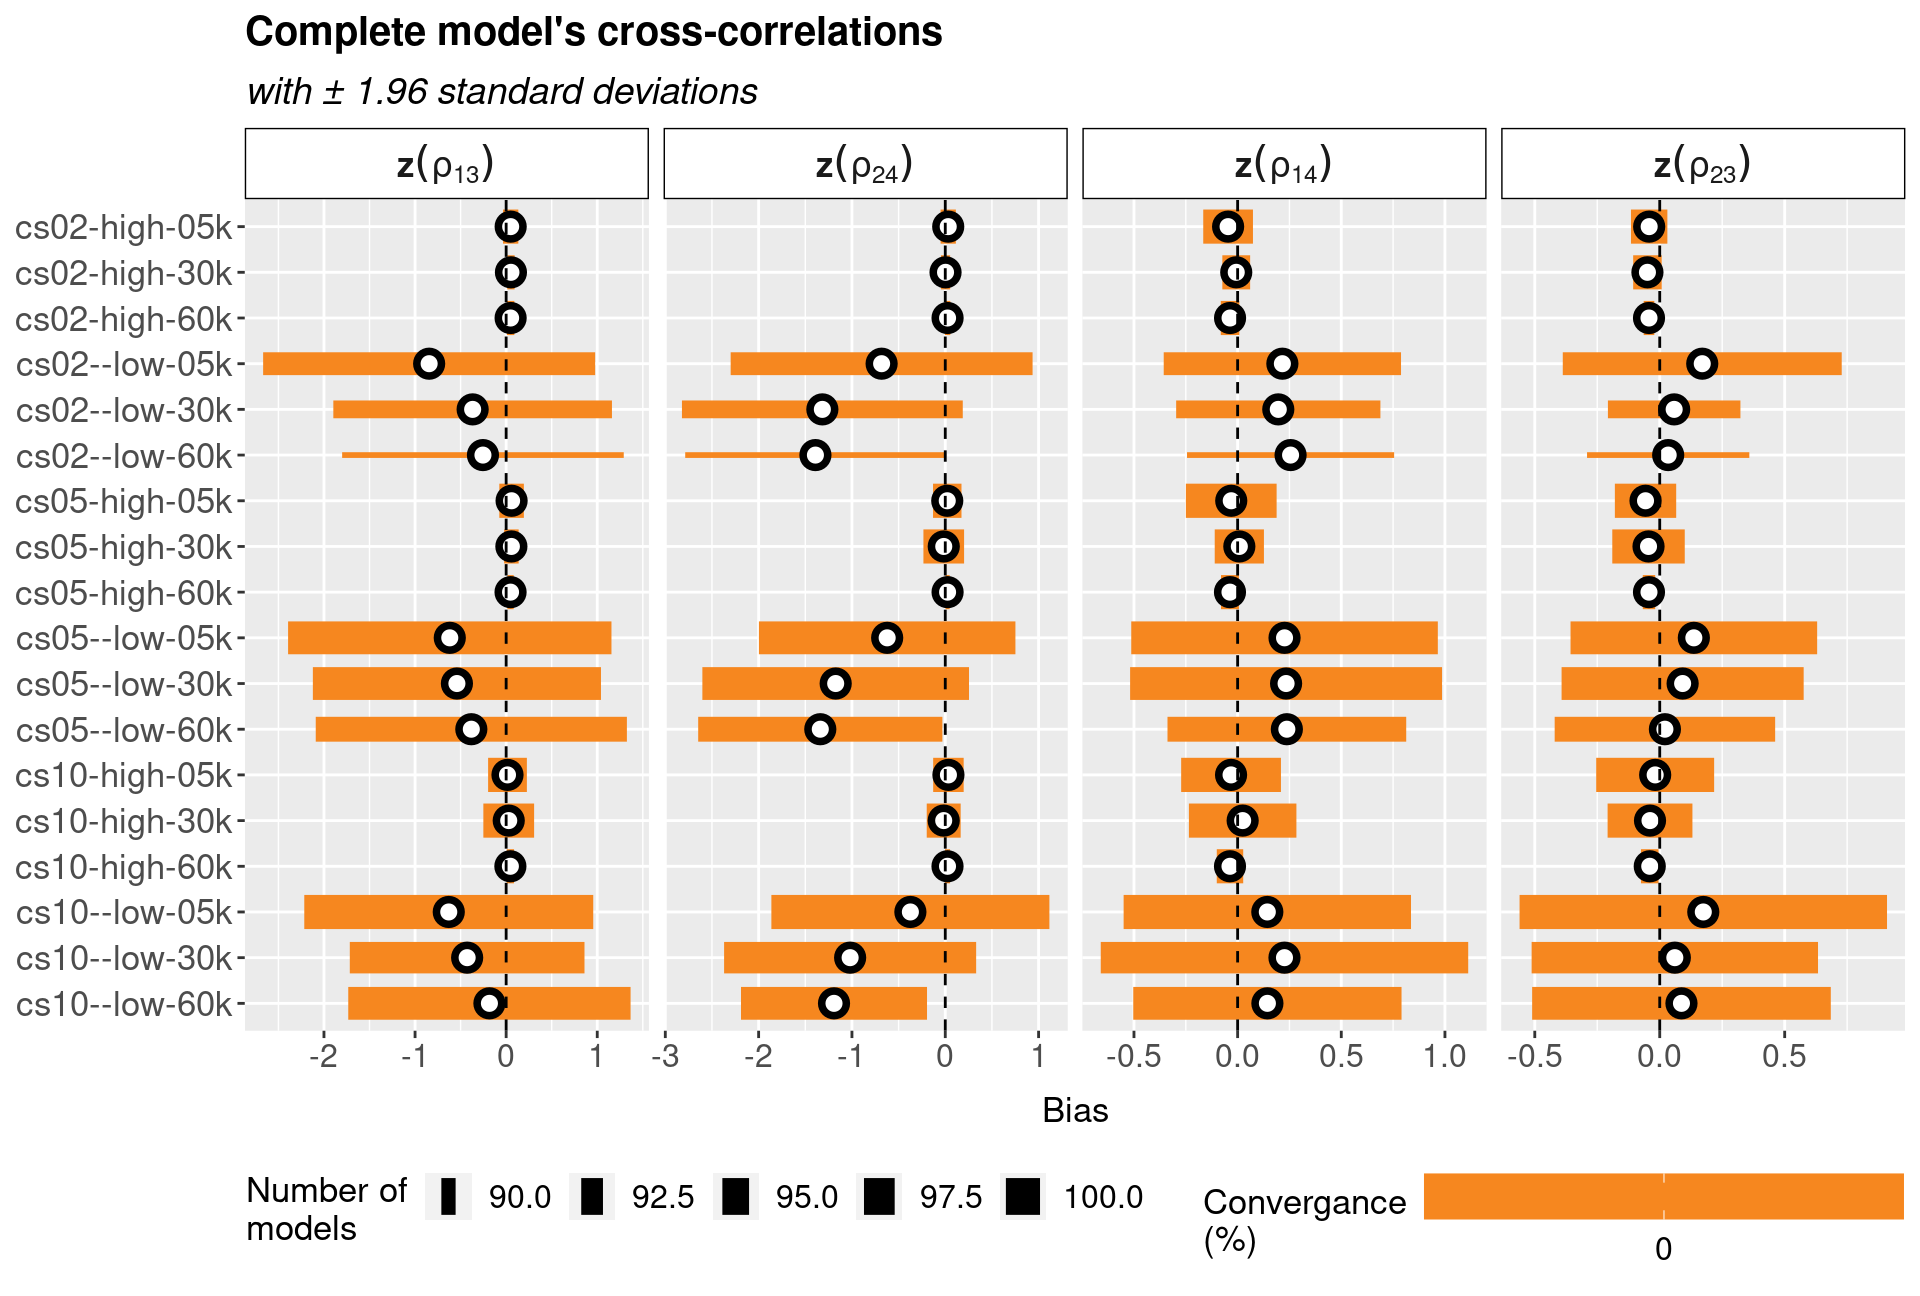
\includegraphics[width=\textwidth]{bias2plotsd-13.png}\\
 \begin{footnotesize}
  SOURCE: The author (2021).
 \end{footnotesize}
 \label{fig:biassdrhoz4}
\end{figure}

\begin{figure}[H]
 \setlength{\abovecaptionskip}{.0001pt}
 \caption{CUMULATIVE INCIDENCE FUNCTIONS (CIFs) HIGH}
 \vspace{0.2cm}\centering
 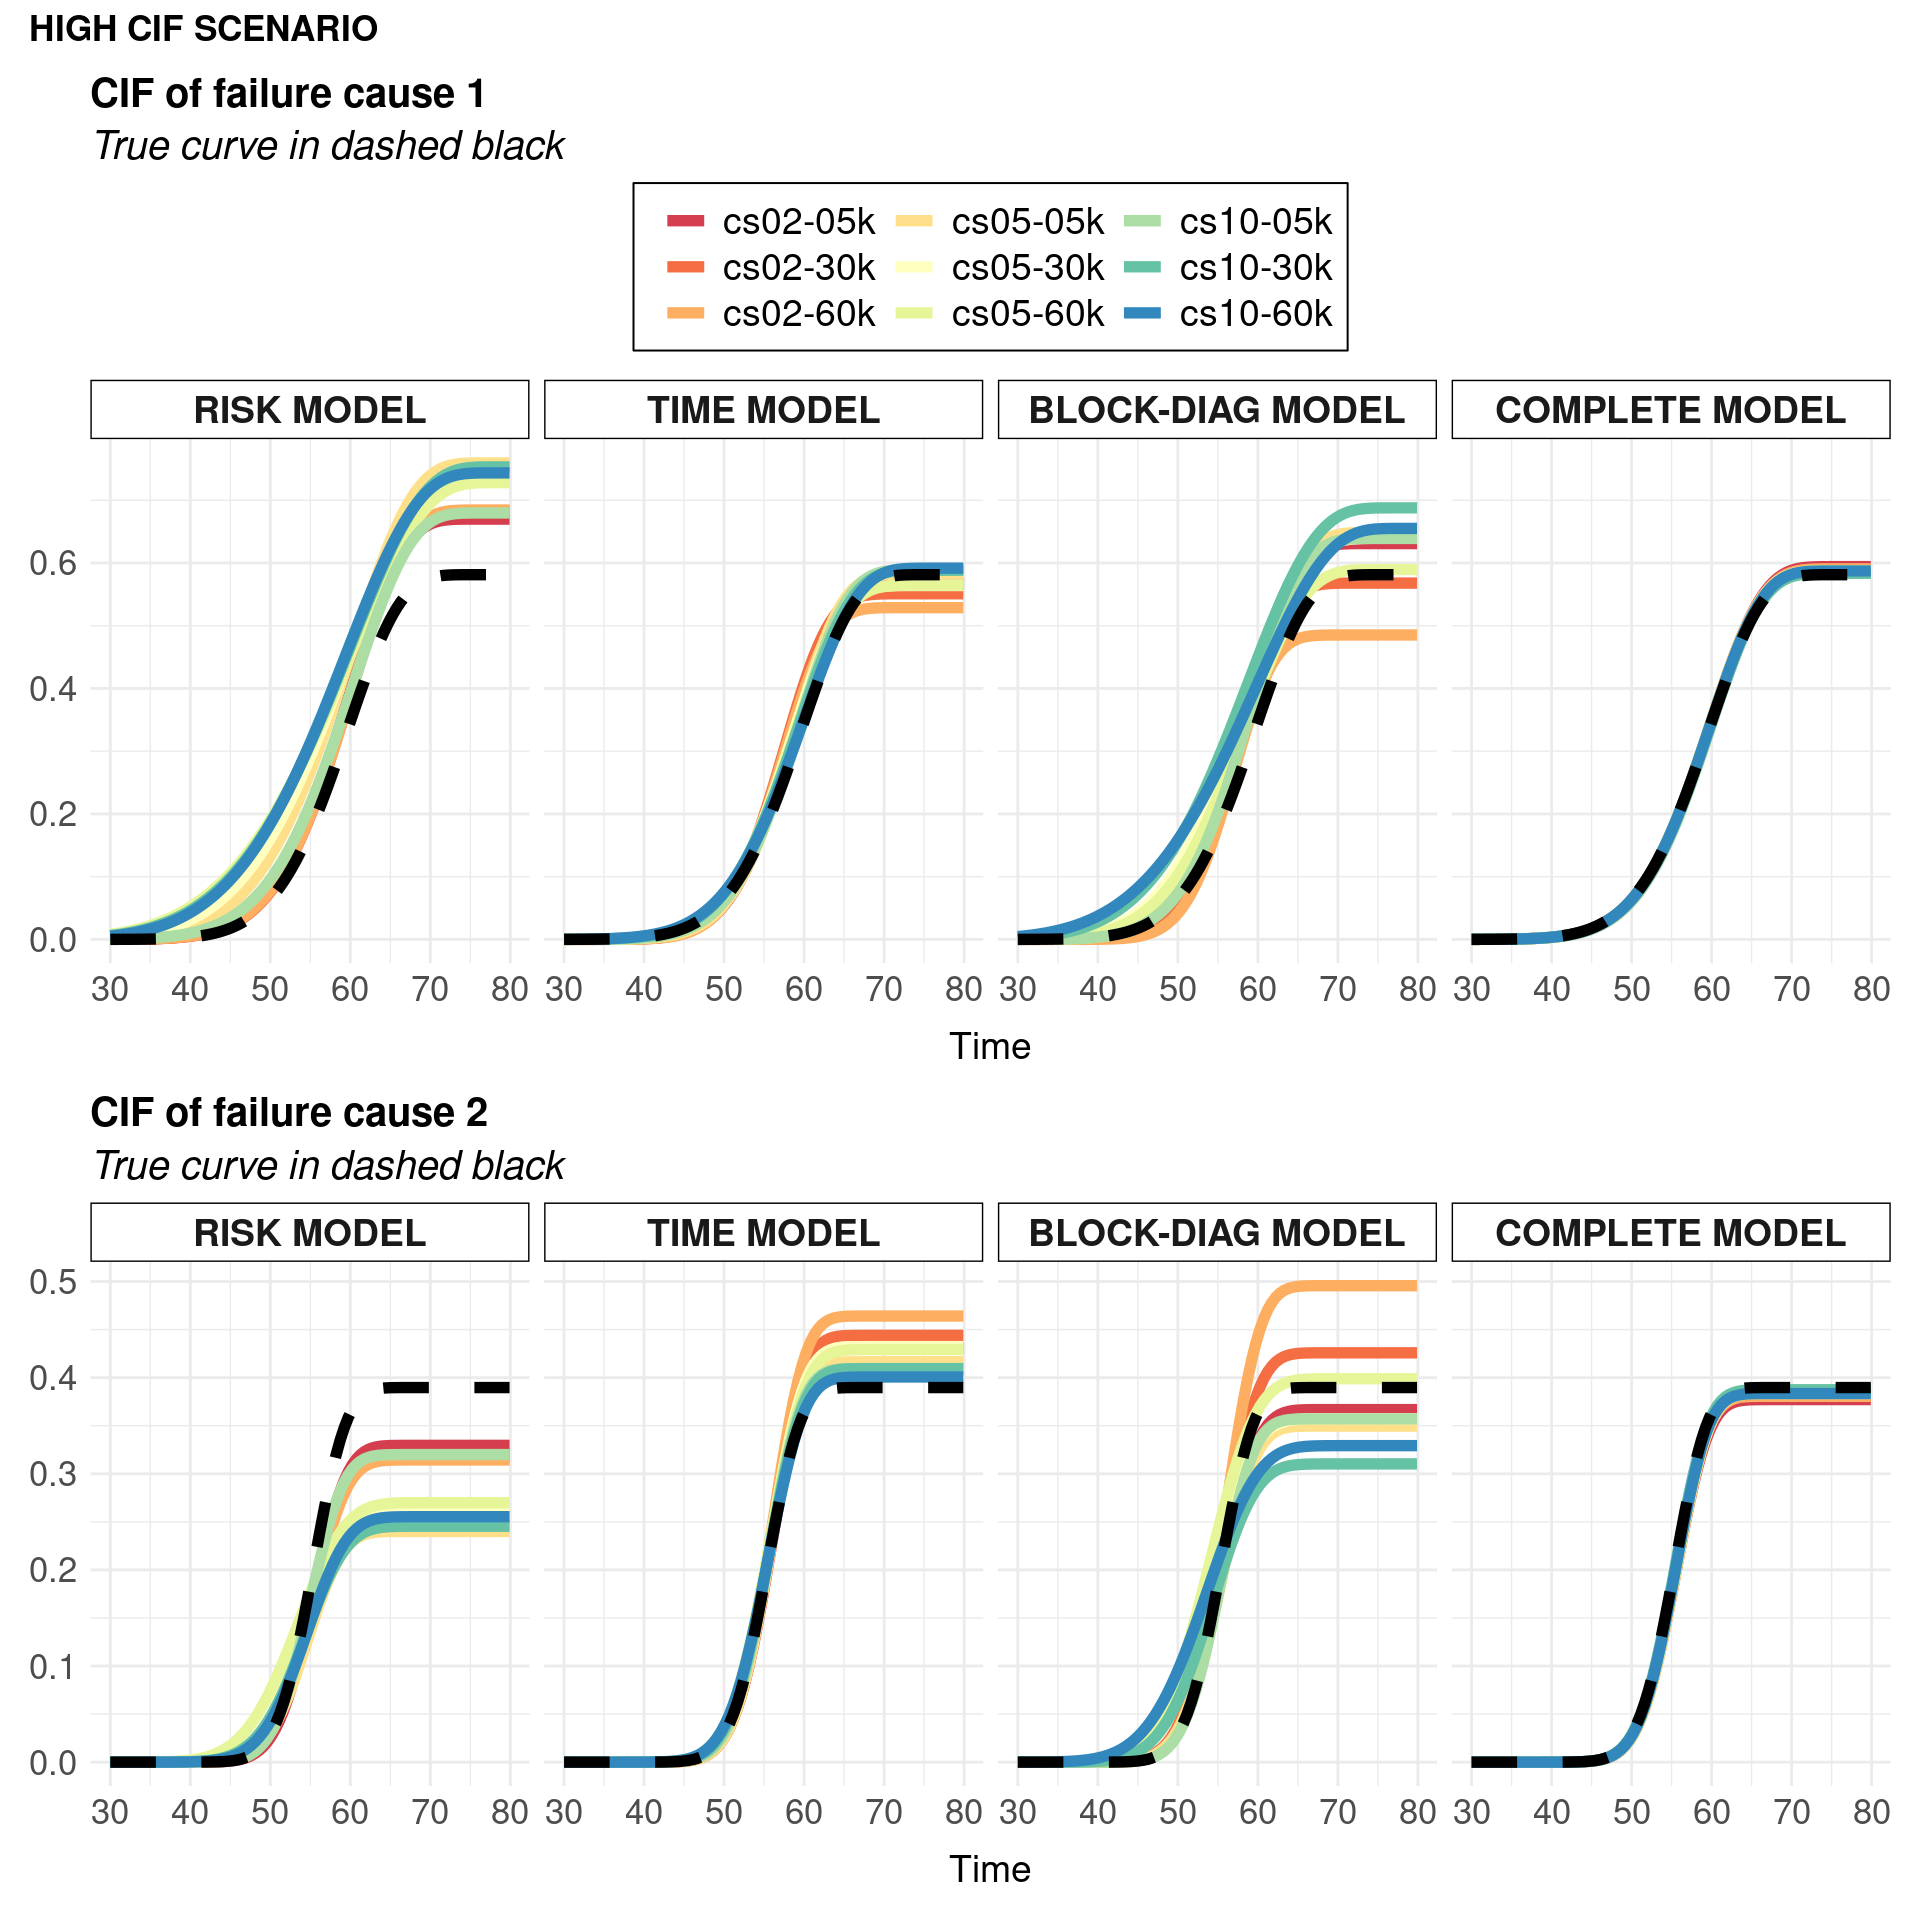
\includegraphics[width=\textwidth]{cifs-1.png}\\
 \begin{footnotesize}
  SOURCE: The author (2021).
 \end{footnotesize}
 \label{fig:cifshigh}
\end{figure}

\begin{figure}[H]
 \setlength{\abovecaptionskip}{.0001pt}
 \caption{CUMULATIVE INCIDENCE FUNCTIONS (CIFs) LOW}
 \vspace{0.2cm}\centering
 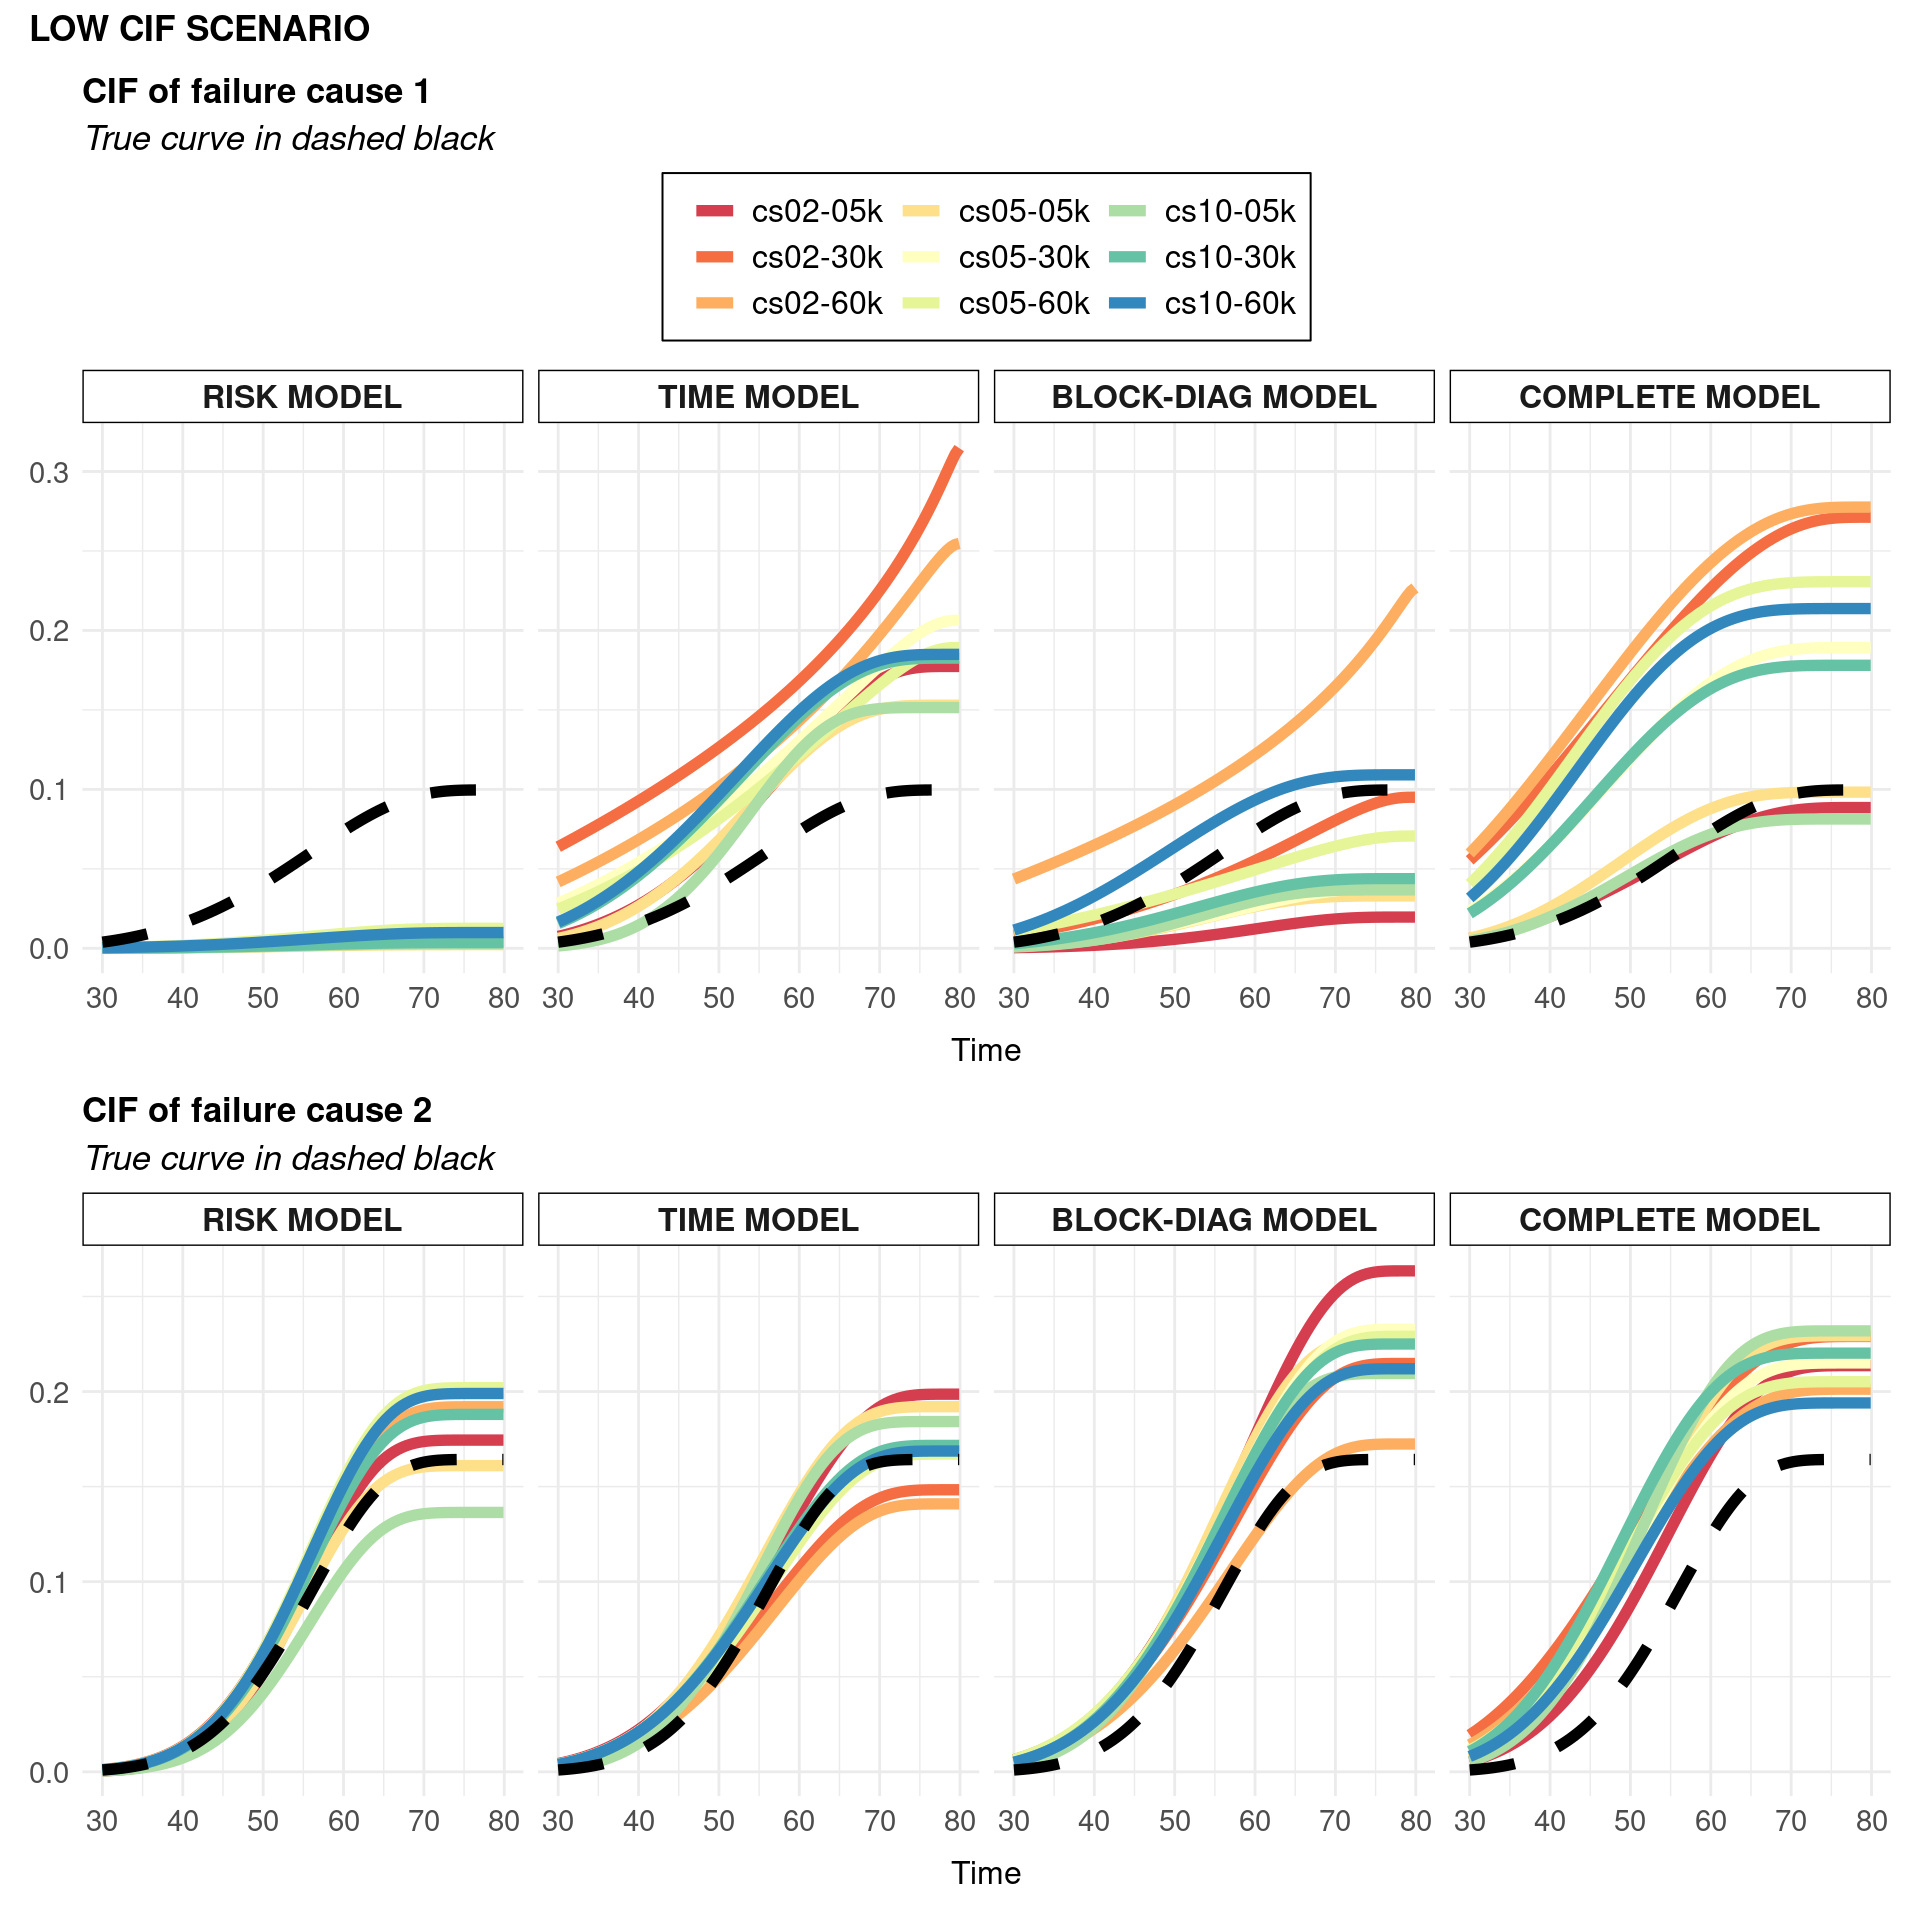
\includegraphics[width=\textwidth]{cifs-2.png}\\
 \begin{footnotesize}
  SOURCE: The author (2021).
 \end{footnotesize}
 \label{fig:cifslow}
\end{figure}

%% \begin{figure}[H]
%%  \setlength{\abovecaptionskip}{.0001pt}
%%  \caption{BUILDING \(\Sigma\)}
%%  \vspace{0.2cm}\centering
%%  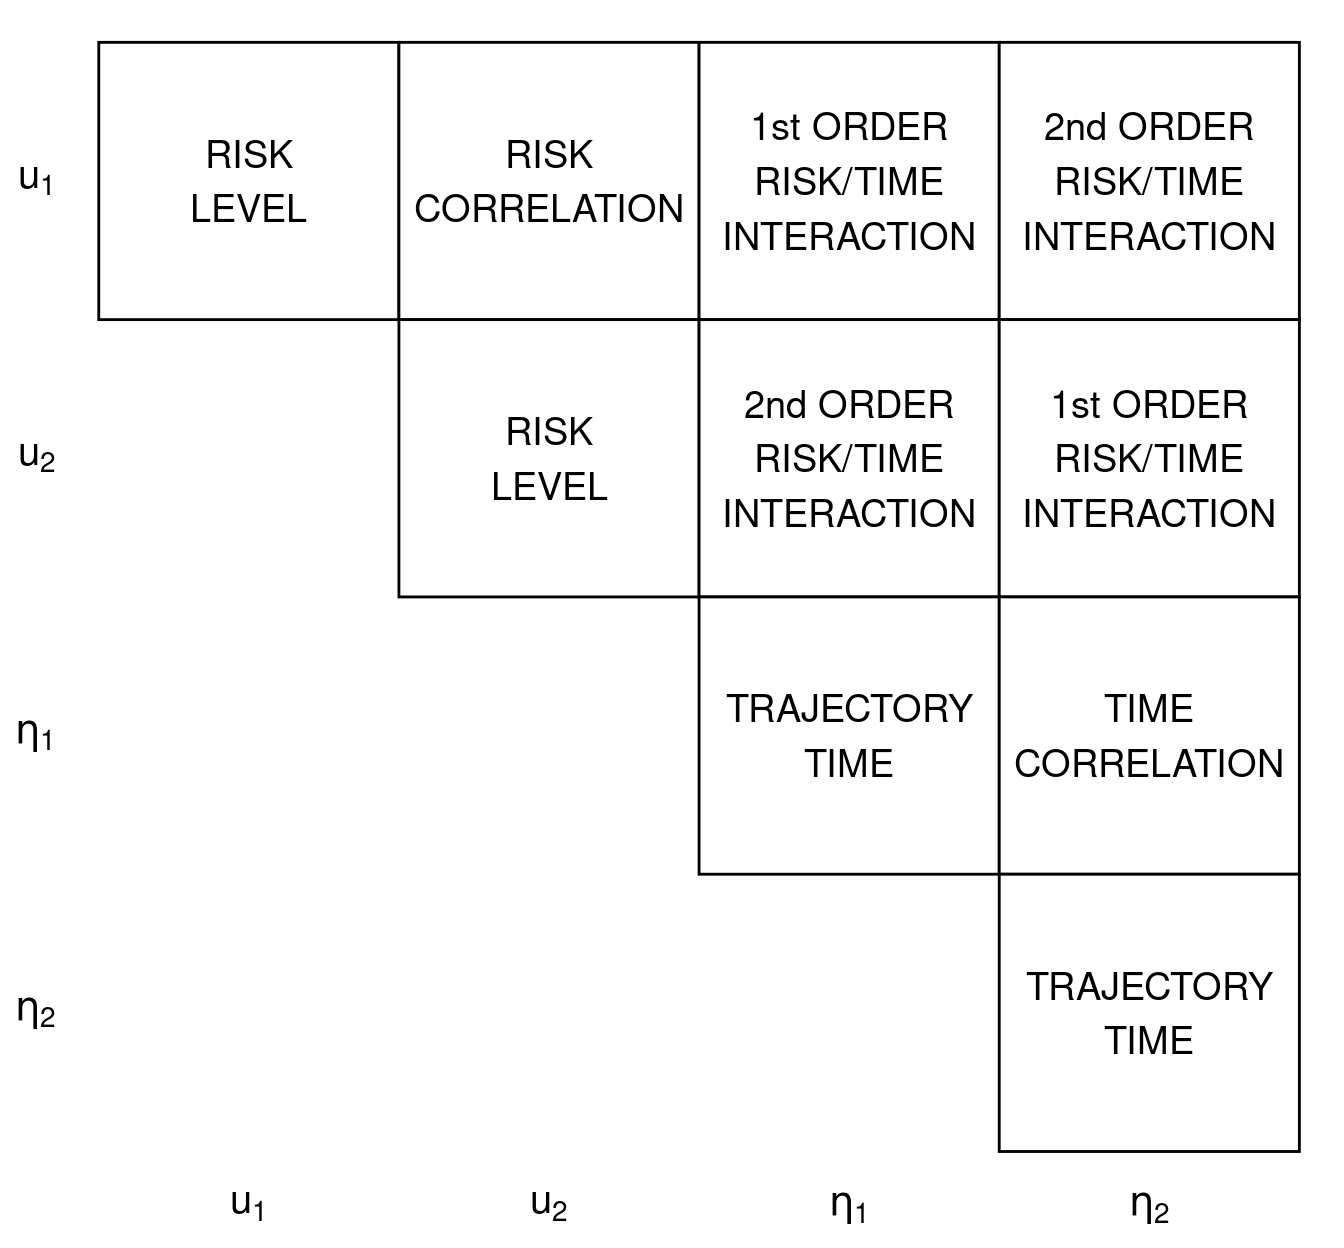
\includegraphics[width=0.75\textwidth]{buildingSigma-1.png}\\
%%  \begin{footnotesize}
%%   SOURCE: The author (2021).
%%  \end{footnotesize}
%%  \label{fig:buildingSigma}
%% \end{figure}

%% \begin{figure}[H]
%%  \setlength{\abovecaptionskip}{.0001pt}
%%  \caption{PARAMETERS CORRELATION}
%%  \vspace{0.2cm}\centering
%%  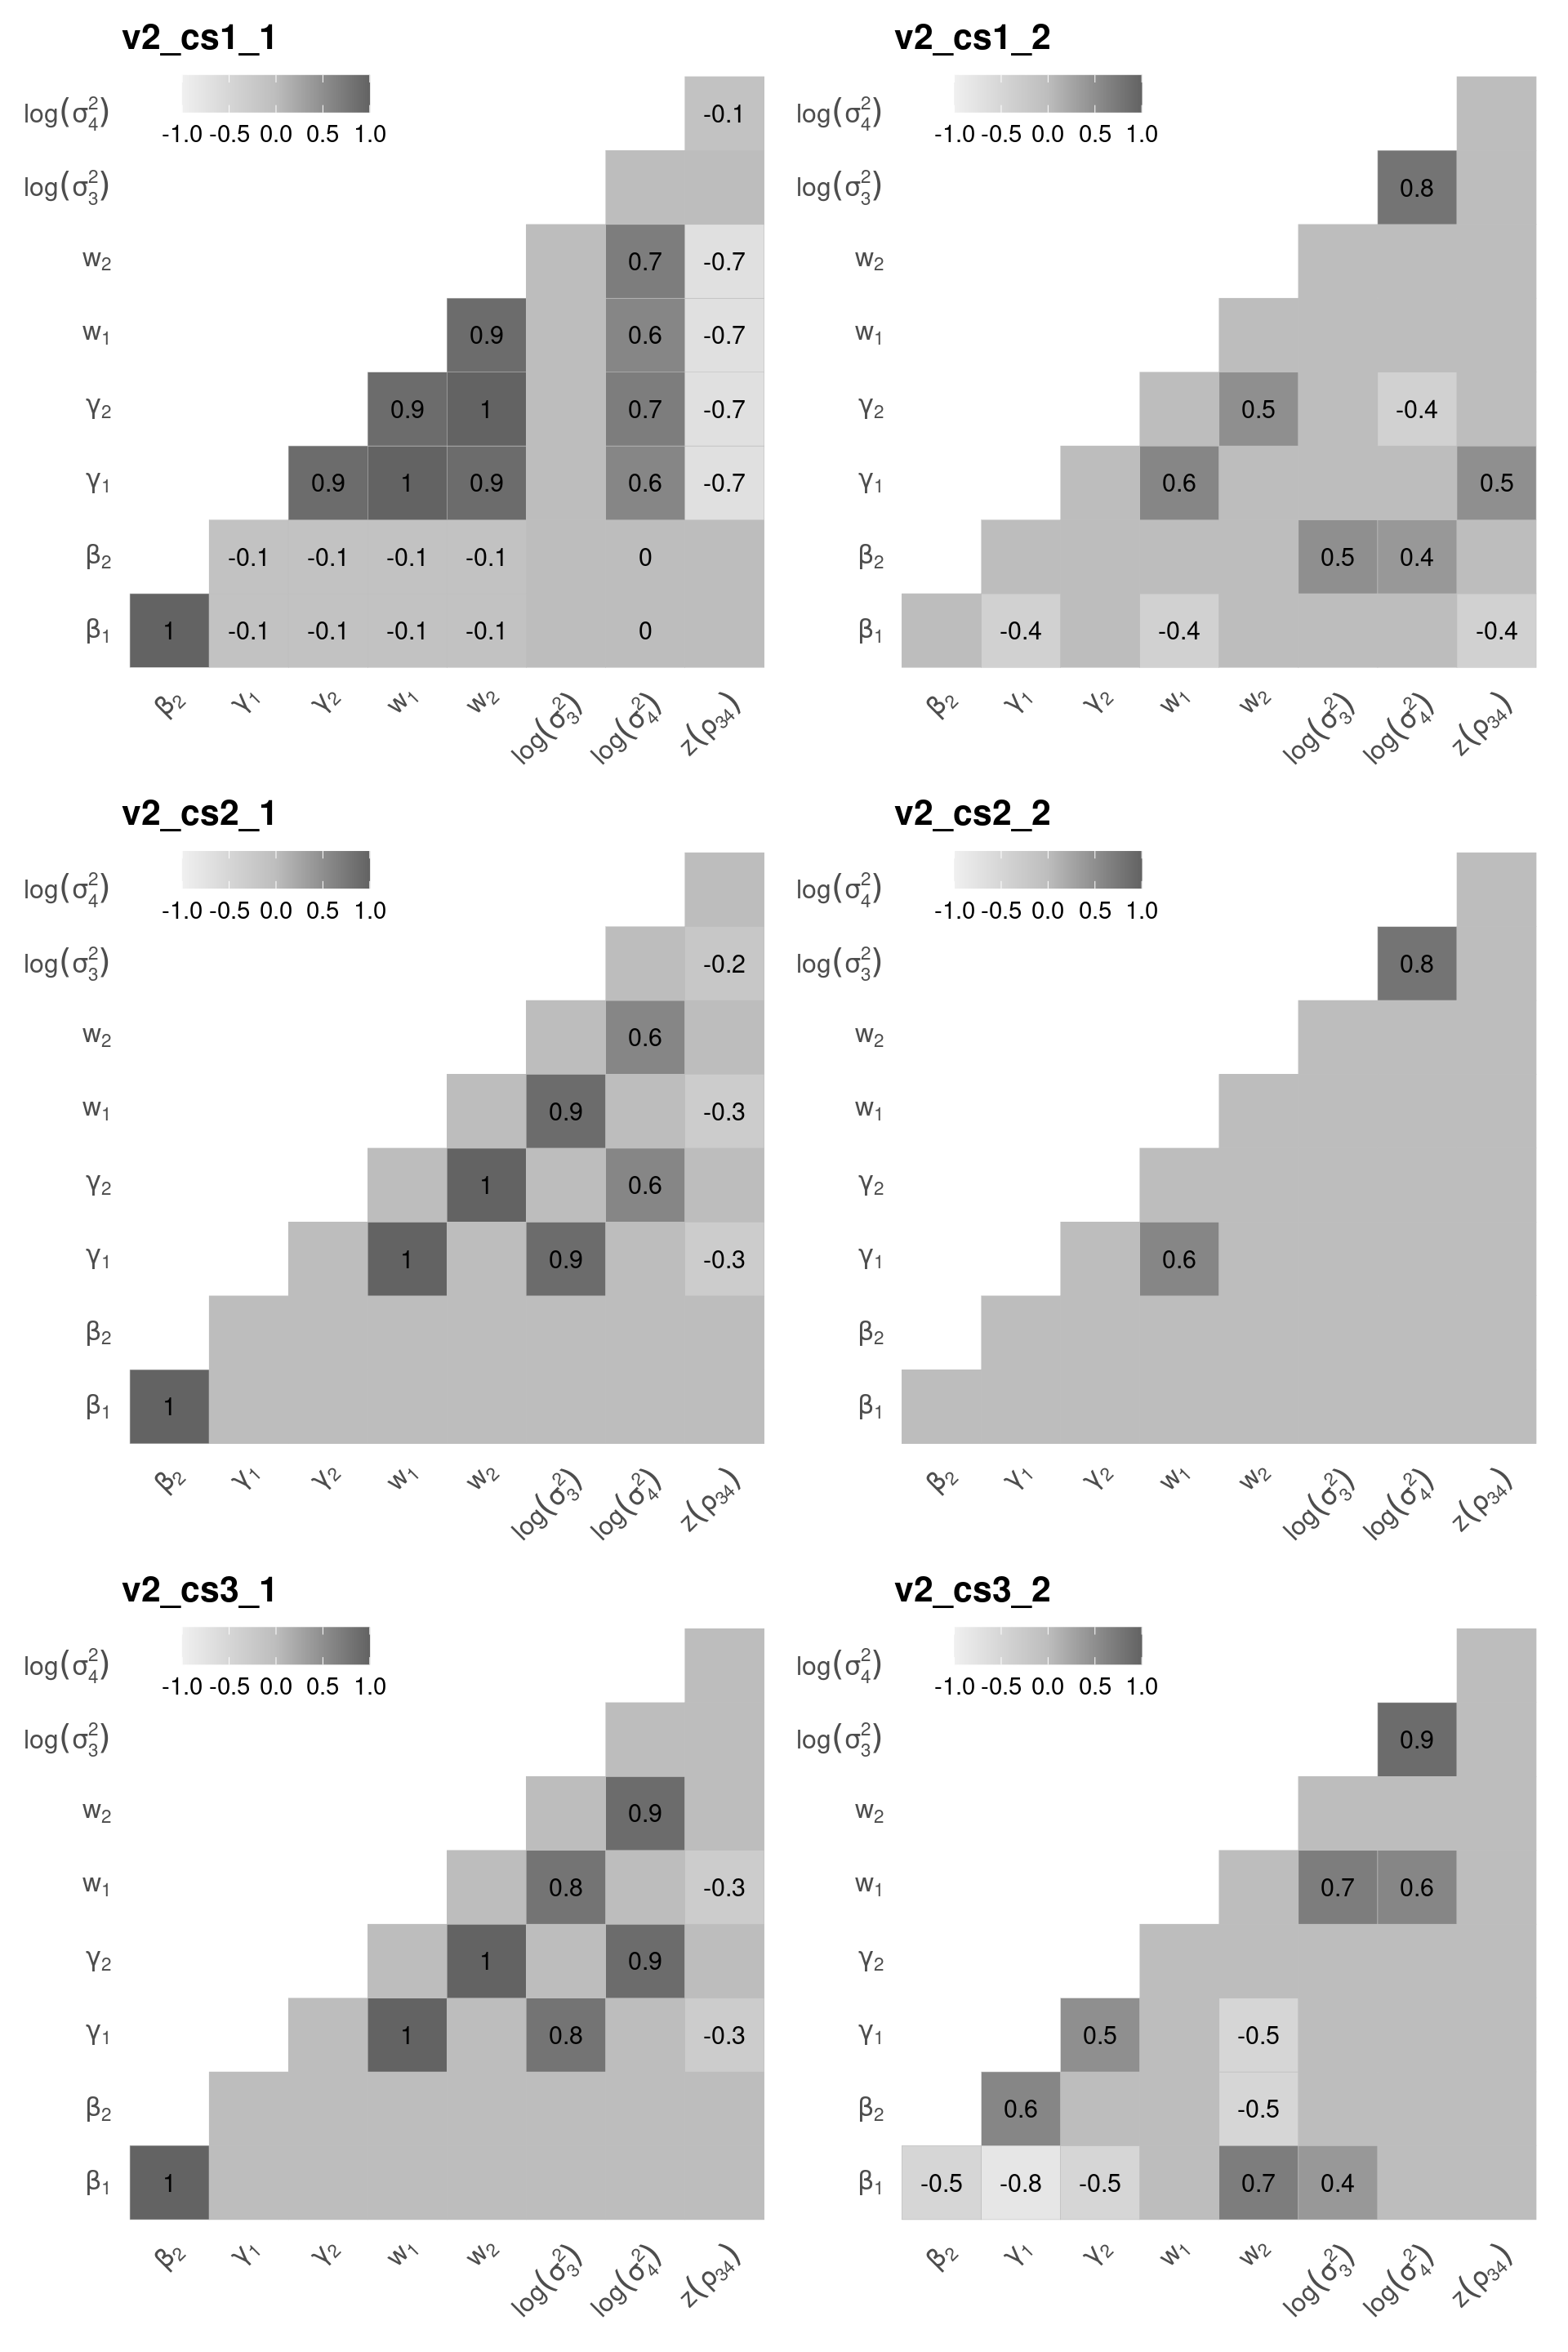
\includegraphics[width=\textwidth]{cor2plot-1.png}\\
%%  \begin{footnotesize}
%%   SOURCE: The author (2021).
%%  \end{footnotesize}
%%  \label{fig:cor2plot}
%% \end{figure}

%% \begin{figure}[H]
%%  \setlength{\abovecaptionskip}{.0001pt}
%%  \caption{VARIANCE-COVARIANCE MATRIX UPPER-TRIANGULAR COMPONENTS}
%%  \vspace{0.2cm}\centering
%%  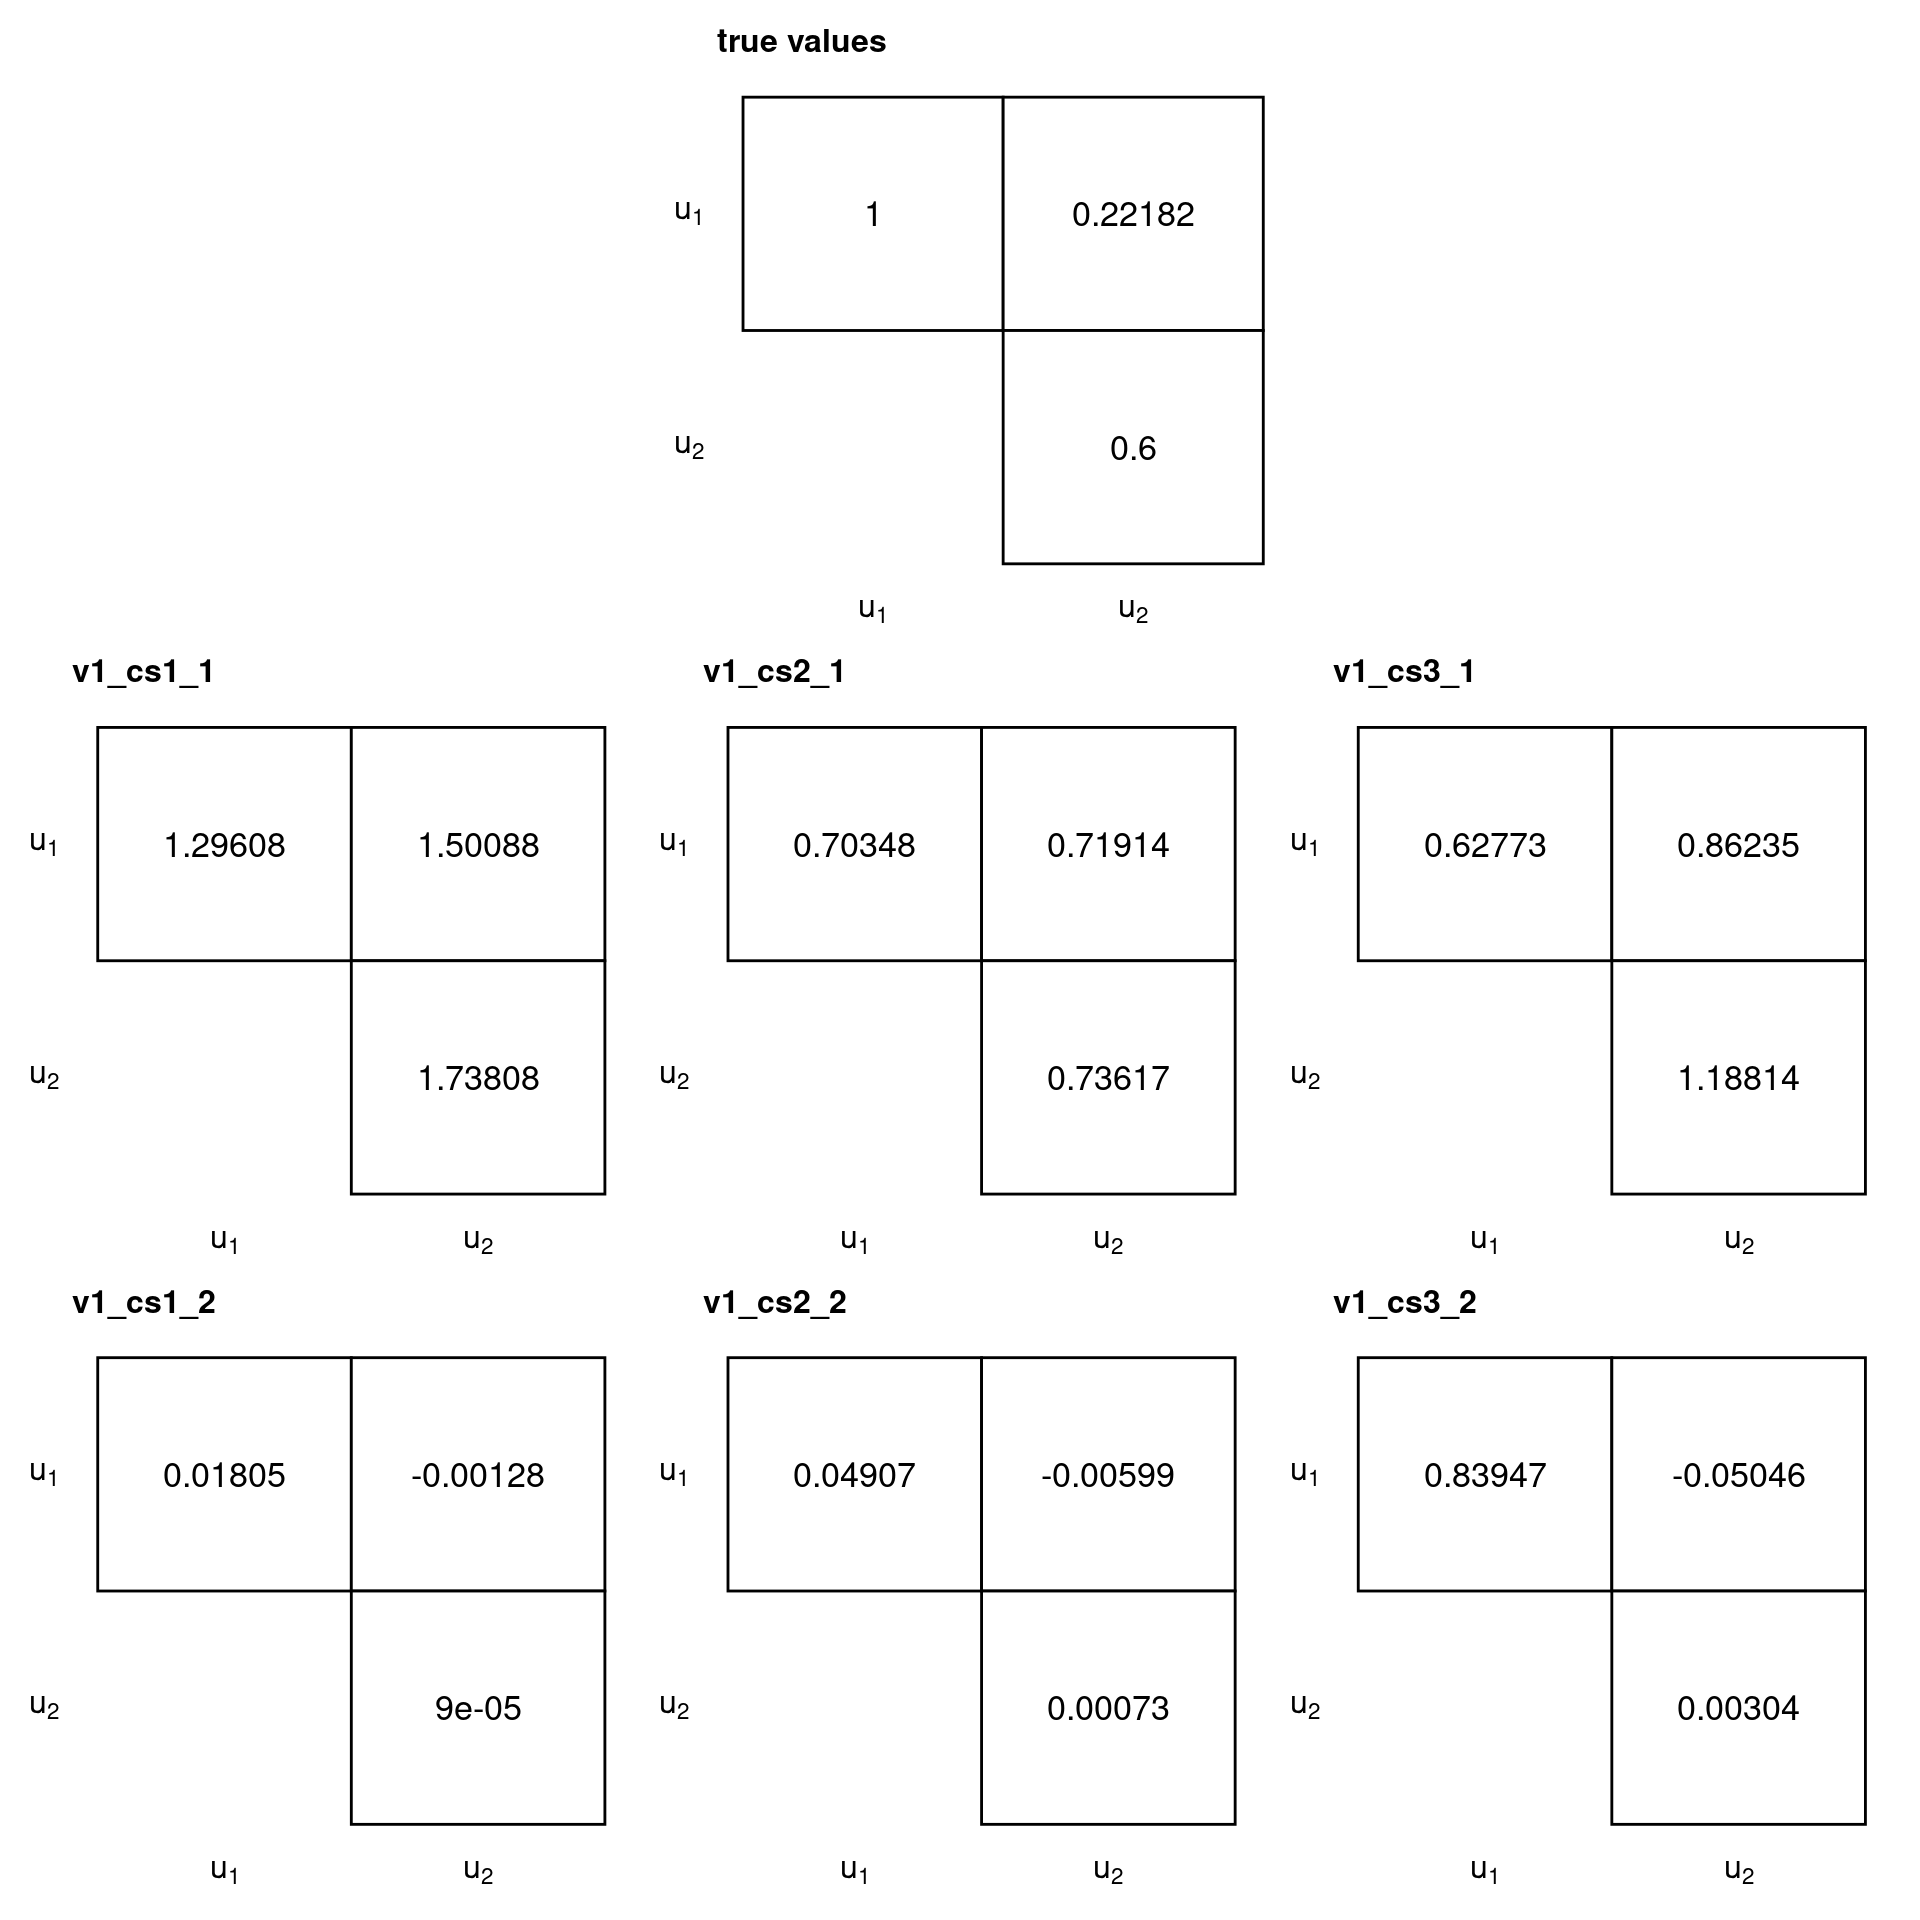
\includegraphics[width=\textwidth]{vcovs-1.png}\\
%%  \begin{footnotesize}
%%   SOURCE: The author (2021).
%%  \end{footnotesize}
%%  \label{fig:vcovs}
%% \end{figure}

% END ==================================================================
